% MIT License

% Copyright (c) 2019-2021 Simon Crase

% Permission is hereby granted, free of charge, to any person obtaining a copy
% of this software and associated documentation files (the "Software"), to deal
% in the Software without restriction, including without limitation the rights
% to use, copy, modify, merge, publish, distribute, sublicense, and/or sell
% copies of the Software, and to permit persons to whom the Software is
% furnished to do so, subject to the following conditions:

% The above copyright notice and this permission notice shall be included in all
% copies or substantial portions of the Software.

% THE SOFTWARE IS PROVIDED "AS IS", WITHOUT WARRANTY OF ANY KIND, EXPRESS OR
% IMPLIED, INCLUDING BUT NOT LIMITED TO THE WARRANTIES OF MERCHANTABILITY,
% FITNESS FOR A PARTICULAR PURPOSE AND NONINFRINGEMENT. IN NO EVENT SHALL THE
% AUTHORS OR COPYRIGHT HOLDERS BE LIABLE FOR ANY CLAIM, DAMAGES OR OTHER
% LIABILITY, WHETHER IN AN ACTION OF CONTRACT, TORT OR OTHERWISE, ARISING FROM,
% OUT OF OR IN CONNECTION WITH THE SOFTWARE OR THE USE OR OTHER DEALINGS IN THE
% SOFTWARE.

\documentclass[]{article}
\usepackage{caption,subcaption,graphicx,float,url,amsmath,amssymb,tocloft}
\usepackage[hidelinks]{hyperref}
\usepackage[toc,acronym,nonumberlist]{glossaries}
\usepackage{titling}
\setacronymstyle{long-short}
\usepackage{glossaries-extra}
\graphicspath{{figs/}} 
% I snarfed the next line from Stack exchange
% https://tex.stackexchange.com/questions
%    /42726/align-but-show-one-equation-number-at-the-end
% It allows me to suppress equation numbers with align*,
% then selectively add equation numbers
% for lines that I want to reference slsewhere
\newcommand\numberthis{\addtocounter{equation}{1}\tag{\theequation}}
\setlength{\cftsubsecindent}{0em}
\setlength{\cftsecnumwidth}{3em}
\setlength{\cftsubsecnumwidth}{3em}
% Ignore garbage that the proprocessor picks up
\DeclareUnicodeCharacter{2192}{~}

% Add logo st start of document
\pretitle{
	\begin{center}
		
\includegraphics[width=6cm]{KanjiLife}\\
	}
	\posttitle{\end{center}}

%opening
\title{
	Notes from Origins of Life\\
	Week 1: Introduction
}

\author{Simon Crase (compiler)\\simon@greenweaves.nz}

\makeglossaries

\loadglsentries{glossary-entries}
% Prefix section numbers with week number
\renewcommand{\thesection}{1.\arabic{section}}
\renewcommand{\glstextformat}[1]{\textbf{\em #1}}

\begin{document}

\maketitle

\begin{abstract}
    These are my notes from the $1^{st}$ week of the Santa Fe Institute Origins of Life Course\cite{sfi2020}.\\
    The content and images contained herein are the intellectual property of the Santa Fe Institute, with the exception of any errors in transcription, which are my own.
    These notes are distributed in the hope that they will be useful, but without any warranty, and without even the implied warranty of  merchantability or fitness for a particular purpose. All feedback is welcome,  but I don't necessarily undertake to do anything with it.\\
    \LaTeX source for all six lectures can be found at\\
    \url{https://github.com/weka511/complexity/tree/master/origins}.
\end{abstract}

\setcounter{tocdepth}{2}
\tableofcontents
\listoffigures

\section[Welcome To The Course]{Welcome To The Course--Chris Kempes}

How life originated is one of the most interesting, complicated, difficult, and still open questions in modern science. Throughout this course, we're going to
introduce to you to why it's such a tricky question, and all the different ways that people are trying to solve this unanswered question.	

Since the time of Darwin, we've come to understand how life progresses, changes, diversifies, finds new niches, evolves greater complexity And yet we still don't understand how to take that back to the original formation and initiation and origin of life.

It's important to recognize that life lives on a spectrum--Figure \ref{fig:lifesTransitions}.

\begin{figure}[H]
	\caption[Life lives on a spectrum]{Life lives on a spectrum, which goes from a completely abiotic world
		all the way up to multicellular creatures like us, and on toentire societies.}\label{fig:lifesTransitions}
	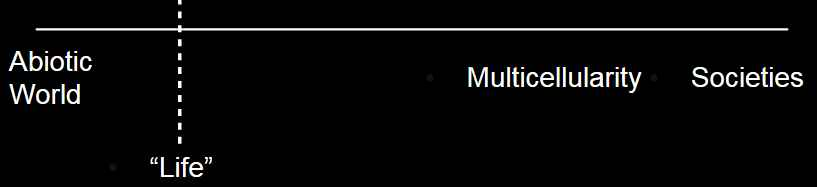
\includegraphics[width=0.9\textwidth]{lifesTransitions}
\end{figure}
At some point along this trajectory, we have this transition into something
that we would call life. How is it that we go from this
abiotic world to a biotic world, understanding that this is all part of one
evolutionary continuum. Why is that question so challenging?

Well, one of the things that makes it challenging is that it requires a lot of diverse types of knowledge to begin to understand this process and to answer this question;those types of knowledge draw from a variety of different disciplines--Figure \ref{fig:tradional:disciplines}.
\begin{figure}[H]
	\begin{center}
		\caption[Traditional disciplines needed for Origin of Life]{We need to understand something about Earth science, biology, chemistry, and physics and how all of these different concept areas intersect with one another and help us to understand exactly what happened when life first formed.}\label{fig:tradional:disciplines}
		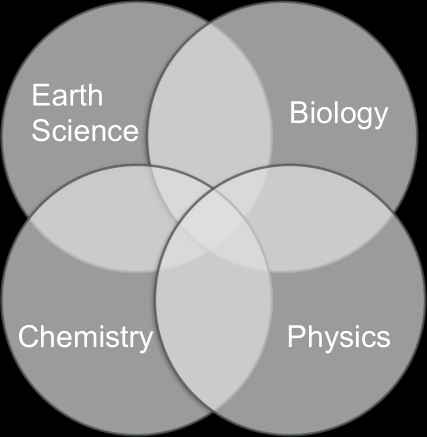
\includegraphics[width=0.9\textwidth]{4mainAreas}
	\end{center}
\end{figure}

Throughout this course, we will introduce you to the main questions in each of these concept areas and how they relate to the origins of life. And we will also start to begin to paint a picture of where the intersection and synthesis of these different concepts live, hopefully moving towards a better theory of how life started and evolved into greater complexity.

What are the main questions within these concept areas? 

\subsection{Earth Science}

\begin{itemize}
	\item What was the environment like during the time when life originated?
	We understand that the early Earth was 	very different from the modern Earth.
	\item What chemistry was possible on the early Earth? We need to understand something about what chemistry was possible then and how that might come together to help 	life form in the first place.
	\item What was the diversity and complexity of various micro-environments on the early Earth? If we think about the early Earth, not only as a different average chemical space from what we currently have, but	also having lots of different unique types of micro-environments in this very different planetary environment, which of those micro-environments were most likely to give us life in the first place or to have the right type of chemical complexity 	to at least start down that trajectory towards a living organism?
	
	\item How did early life and the geosphere co-evolve? 
	We understand, in the modern Earth, how life interacts with the overall planetary	system; we understand, through lots of the history of life how life interacts, has a large feedback width, and modifies	the geological environment and the geosphere. And the question is: when life first started, what did	that feedback look like and how did this coevolution happen, and how important was that for the	specific trajectory that life took once it was formed?
\end{itemize}


\subsection{Biology}
\begin{itemize}
	\item How do we wind the clock back from modern life to early life? From a biological perspective, the questions we're interested in are mostly how do we take everything we know about modern life and try to work as far back in time as we can? How do we wind back the clock on modern life to understand what early life might have looked like?
	This involves taking a lot of phylogenetic or genetic perspectives to
	look back in time.
	\item  What does the composition, structure, and function of modern life tell us about the origin?
	\item  Which aspects of extant life are general and which are arbitrary?
	\item How do we apply modern evolutionary theory to the proto-life? Also in that vein, how do we take everything we know about modern evolutionary theory and start to apply that to things like protolife which might have a much less formal version of
	inheritance or genetics.
	\item How can we use evolutionary theory to think about the simplest early life which
	might be radically different but also is almost certainly undergoing some sort of
	evolutionary process. So, what are the features that we see in 	modern life that are really essential to life through any origin and trajectory and 	which are contingent on the particular evolutionary history that we happened to
	have seen for more recent life?
\end{itemize}	


\subsection{Chemistry}
\begin{itemize}
	\item How does life arise from the huge space of chemical reactions and compounds? 
	We understand that chemistry gives us 	this really vast set of possibilities, 	this really rich high-dimensional space, which is great for allowing something 	like life to form but it makes it very complicated to understand exactly what combinations and processes and trajectories are actually necessary or were the ones that led to the life that we have.
	\item What was early “living” chemistry like? How was that possible in early Earth? How do 	we start to define sort of living chemistry that isn't quite life?
	\item How do we go from complicated chemistry in an environment to the amazing chemical complexity of even the simplest cells? Even the simplest cells have a set of chemistry and feedback and dynamics and interconnections that is much more 
	complicated than things that we see in the environment and so how do we make that
	transition?
\end{itemize}

	
\subsection{Physics}

\begin{itemize}
	\item How do physical constraints, such as the laws of thermodynamics, bound the possibilities for life? How do we take everything we know about physics and use that to say what is and 	isn't possible for life, especially for the	first forms?
	\item What properties and processes are ''easy'' to obtain through physical dynamics alone?	So for example, we understand that in 	purely physical systems, it's possible to get very rich pattern information and 	dynamics and so how much-- how important 	are those sorts of naturally emergent--	occurring phenomena to thinking about the first formation of life and how we start 	to apply some of those concepts of 	emergence and simple pattern formation to 	interact with
	how life began in the first place.
	\item How do we generalize physical concepts to understand life’s formation? How do we port physical concepts over 	to biology in general and in particular, how do we port those ideas over to the origins of life?
\end{itemize}	

As you can see this is a very rich set of questions coming out of a variety of concept spaces across a huge range of science and in this course we've gathered people from this wide diversity of scientific perspectives to really lay out the details of each of these questions in specific ways and then bring those details together in a way that we have a broader and more complete understanding of how life might have formed in the first place.


\section[Life]{Life--David Baum}

\subsection{Easy or hard?}
A key initial consideration is how easy, or hard, is it for life to emerge?
The extremes:
\begin{itemize}
	\item We need to wait billions of years for specific conditions: even hospitable planets lack life--Figure \ref{fig:luca}.
	\item New life can evolve quickly whenever conditions are ripe:  New life could emerge in the lab--Figure \ref{fig:zircons}.
\end{itemize}

Of course this isn't really a dichotomy, as there is a continuum from easy to hard.

\begin{figure}[H]
	\caption[Life is hard.]{Life is hard; Time is long. A key piece of evidence comes from looking at cellular life and tracing it back to a single ancestor--\gls{gls:LUCA}. If life were easy one might expect multiple independent trees.}\label{fig:luca} 
	\includegraphics[width=0.9\textwidth]{Luca}
\end{figure}

\begin{figure}[H]
	\caption[Life emerged quickly]{Life emerged quickly: The oldest rocks that could have retained evidence of life do have evidence of life. We now don't know any rock formation that doesn't have evidence of life. This figure depicts some inclusions in zircons\cite{bell2015potentially}, and the isotopic ratios suggest the carbon was from life.}\label{fig:zircons} 
	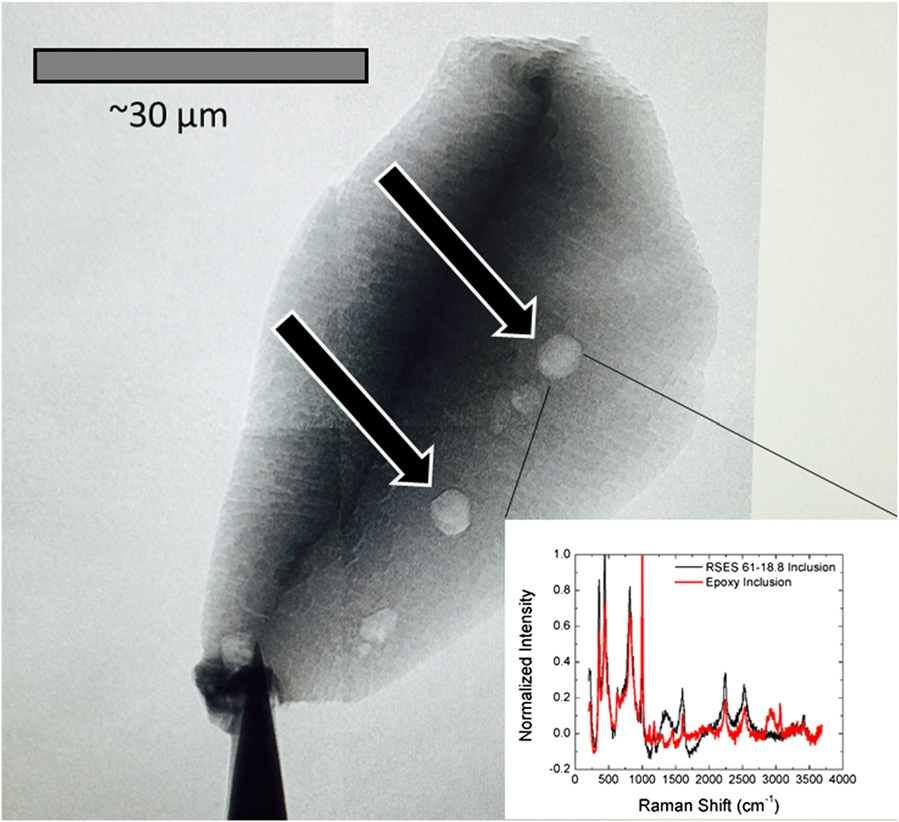
\includegraphics[width=0.9\textwidth]{Zircons}
\end{figure}

 Even if life arose only once, it nevertheless happened remarkably early, since Figure \ref{fig:zircons} dates from shortly after the planet had cooled enough to provide liquid water. To help us think about that we can turn to Charles Darwin.
\begin{itemize}
	\item Life pre-empts Life: \begin{quotation}
		But if (and oh! what a big if!) we could conceive in some warm little pond with all sorts of ammonia and phosphoric salts,—light, heat, electricity etc present, that a protein compound was chemically formed, ready to undergo still more complex changes, at the present day such matter would be instantly devoured, or absorbed, which would not have been the case before living creatures were formed--Charles Darwin\cite{darwin1871letter}. 
	\end{quotation}So the fact that life only emerged once does not necessarily mean that life is hard.
	
	\item Do we know that all life on this planet is cellular? Would we recognize alt-life?
	
	\item Some theories allow life to originate easily\cite{wachtershauser1988before}
\end{itemize}

\subsection{The meaning of ''life''}
In everyday discourse the term "life" is not ambiguous.
When we point at something and label it "alive," or an "instance of life," we usually know what we mean.
But, when it comes to the science and the philosophy of life, this is not so trivial.
And, in fact, scientists and philosophers have debated for a long time what we really mean by the term "life."

And, of course, we have a very clear reference point.
The reference point is cellular life--\gls{gls:LAWKI} on this planet,
which shares a number of distinctive features.
And, we can make a very long list of the features that all life as we know it share, and some of them are very specific.

\gls{gls:LAWKI} shares many features
\begin{itemize}
	\item They all use a nucleic acid code 	with the same bases-- (A,T/U,C, G)
	\item they all use the same 20 amino acids 	to make their proteins;
	\item they're always the left-handed variants.
	\item they will have a very similar genetic code,
	\item they all have similar machinery--ribosomes--for making proteins,
	\item they have similar biochemistry, (e.g. \gls{gls:ATP})
	\item they even share particular genes.
\end{itemize}

It's kind of exciting to realize that all life has these unique
and shared properties, because it tells us something fundamental about life as we know it, which is that life as we know it traces back to a single common ancestor--Figure \ref{fig:LUCA_common}.
\begin{figure}[H]
	\caption{Life as we know it traces back to a single common ancestor}\label{fig:LUCA_common} 
	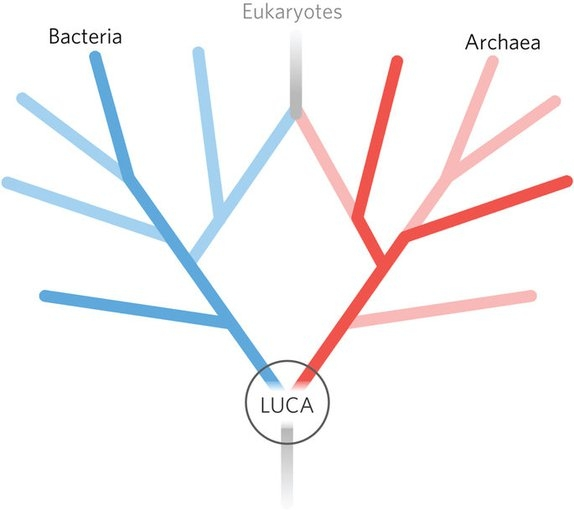
\includegraphics[width=\textwidth]{LUCA_common}
\end{figure}
So, there was, at some point in the past, an ancestral lineage that gave rise to
all three branches of life that we know of today--bacteria, archaea and eukaryotes.

And, the traits that we see in all life as we know it--that list I just gave you and more--all predate the last universal common ancestor, the last organism that was ancestral to all three of those lineages.
So, that's an exciting and important insight, but it also poses a slight problem, which is--life as we know it has a very long list of shared traits.
But, it doesn't necessarily guide us as to ask the question--suppose you found some other lifelike system,maybe on another planet or in some strange environment,you wanted to decide--''Is this thing alive? Is it an instance of life?''--you presumably wouldn't care about this full laundry list.These particular traits are the result of the historical factors that occurred in the origins of this life. and we want some more general understanding of life to answer the question - is something else another instance of life?

So, people have tried to approach this by whittling down those specific traits
to generalities -- general features -- that life seems to have
that distinguish these instances of life from instances of non-life --
inanimate matter. And if, you open any sort of biology textbook, you'll have a list of the features of life, and they vary in number from five, seven, eight, whatever--Figure \ref{fig:lawki-focus}.

\begin{figure}[H]
	\caption{Focus on generic features...but which?}\label{fig:lawki-focus} 
	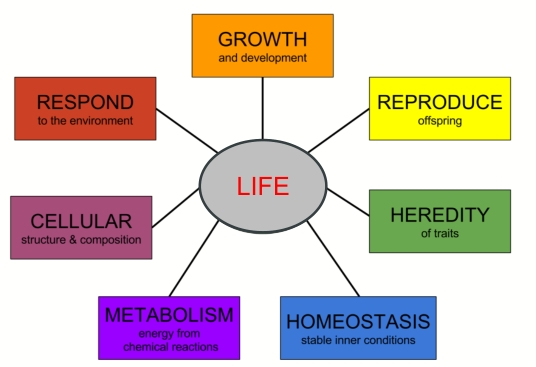
\includegraphics[width=\textwidth]{lawki-focus}
\end{figure}
And, this has been the starting point for a process in the origin of life field of thinking about - how low can we go? 
What, at core, are the essential features of something to be considered to be an instance of life in the general sense?

Now, there might be some difference of opinion, but, by and large, the field has converged on two key features, which are captured in this definition I've given here.
\gls{gls:life} is \glsdesc{gls:life}.

This definition is based on one that was kind of established by NASA to help guide them in the question of looking on other planets and deciding whether there is life there.

\begin{itemize}
	\item life is a self-propagating chemical system, meaning it's a system that makes more of itself over time--or least can;
	\item  we expect  that this system 	is capable of undergoing
	adaptive evolution--Figure \ref{fig:AdaptiveEvolution}.
	\item \emph{self-propagation} and \emph{evolution} are key
\end{itemize}

So, let's look at those two pieces in turn.


The idea of self-propagation is that you have some kind of chemical system that can make more of itself and occupy additional areas of space. It doesn't much matter whether we're thinking about growth, which is where we have a single, living protoplasm that expands to encompass more space, or if we're thinking about the process of making multiple cells from a single parent cell.
The only difference between these phenomena is whether or not the newly formed protoplasm--living material --either is not sort of packaged up into cells.
And so, what we expect of anything that we would label to be "alive"--is that it has some capacity to propagate itself spatially.
But, of course, that isn't really enough because we know of quite a few systems that can self-propagate,
but we usually wouldn't call them "alive"--for example, a crystallization process.
\begin{figure}[H]
	\caption[Adaptive Evolution]{Adaptive evolution entails the potential to complexify and become more out-of-equilibrium. Surface \gls{gls:protoplasm} ulimately evolves to a \gls{gls:protocell}, as described in \cite{baum2015selection}}\label{fig:AdaptiveEvolution} 
	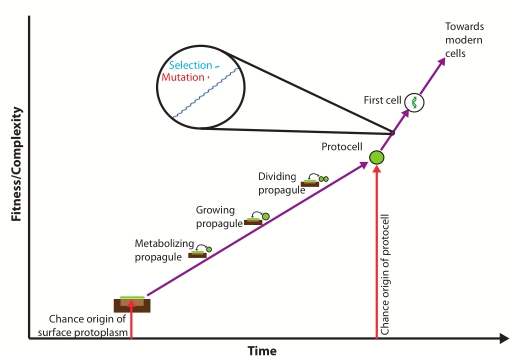
\includegraphics[width=0.9\textwidth]{AdaptiveEvolution}
\end{figure}

And, that's where the second part
of the definition comes in -
and that is this idea that things
that we want to consider to be alive
also have the capacity
for adaptive evolution...
which means that
they have the capacity
to get better at
self-propagating over time.
This is an important idea
and something that we don't see in,
for example, crystallization processes,
because it explains
how it is that life as we know it
became so complicated
and out of equilibrium
with their chemical environments.
Cells and living systems that we know
are quite sophisticated
and certainly far from being typical of
the chemical environment around them.
And, this is possible because,
during the adaptive process,
the variants arise,
and the fate of those variants
is independent of whether they are
of raised or lower complexity.
Natural selection,
the driving force of adaptive evolution,
will select the trait that
confers higher fitness
whether or not
it's a more complicated trait.
Furthermore, there are many instances
in which we know
that the more complicated variants
have an advantage.
As a result,
over long, long periods of time,
adaptive evolution can explain
how a simple self-propagating system
can become more and more complex.

So, putting these
two pieces together,
it's fair to say that
the origin of life field,
in general, has a great deal
of attention...
that it pays to these two properties -
self-propagation and adaptive evolution.
We try and understand
how they come about,
and we try and understand the kinds
of planetary or chemical conditions
in which we might expect
self-propagation and evolution
to emerge spontaneously.



\section[Constraining Chemical Complexity to Form Life]{Constraining Chemical Complexity to Form Life--Zach Adam}

We'll be talking about huge chemical complexity, and constraining the complexity to form life. When we look at the deep past we find some interesting challenges regarding how life could have originated from a non-living environment. Most matter isn't alive: how to bridge the two states of matter?

\begin{figure}[H]
	\caption{Chemical Complexity}\label{fig:ChemicalComplexity} 
	
	\begin{subfigure}[b]{0.45\textwidth}
		\centering
		\caption{When we first learn chemistry, we use stick and ball model}
		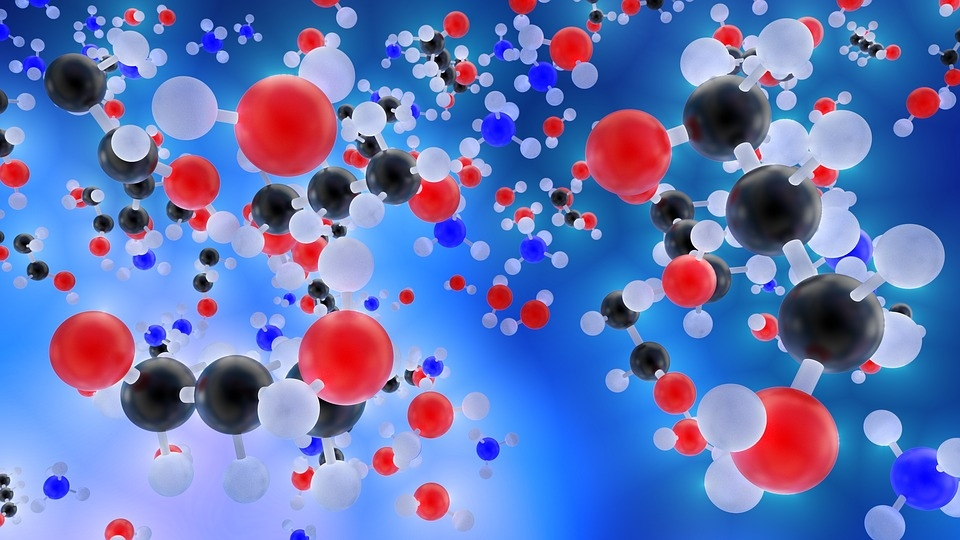
\includegraphics[width=\textwidth]{ChemicalComplexity}
	\end{subfigure}
	\begin{subfigure}[b]{0.45\textwidth}
		\centering
		\caption{But atoms really have many levels, all interacting. The outer layers of electrons give rise to the "sticks" in the na\"ive model.}
		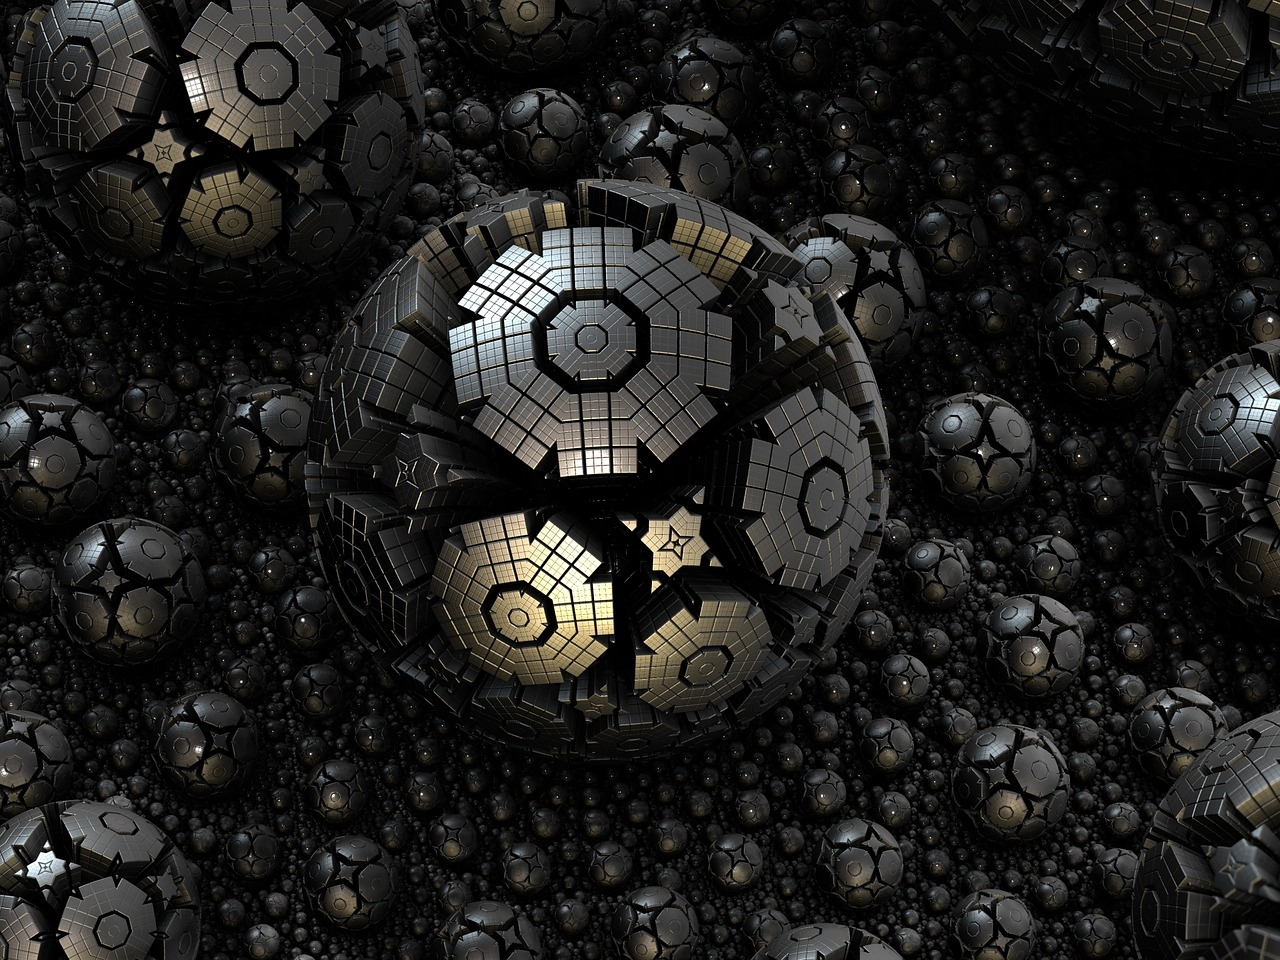
\includegraphics[width=\textwidth]{ChemicalComplexity1}
	\end{subfigure}
\end{figure}

Let's start with a canonical type of molecule--Figure \ref{fig:NucleotideMolecule}. When we zoom in a bead we see that it represents three molecules. If we change even one atom, or link the atoms differently, the molecule may not function.
\begin{figure}[H]
	\caption{Nucleotide Molecule }\label{fig:NucleotideMolecule}
	
	\begin{subfigure}[b]{0.45\textwidth}
		\centering
		\caption{RNA Molecule: one bead expands to 3 molecules. Change one atom, likely to change behaviour of entire molecule!}
		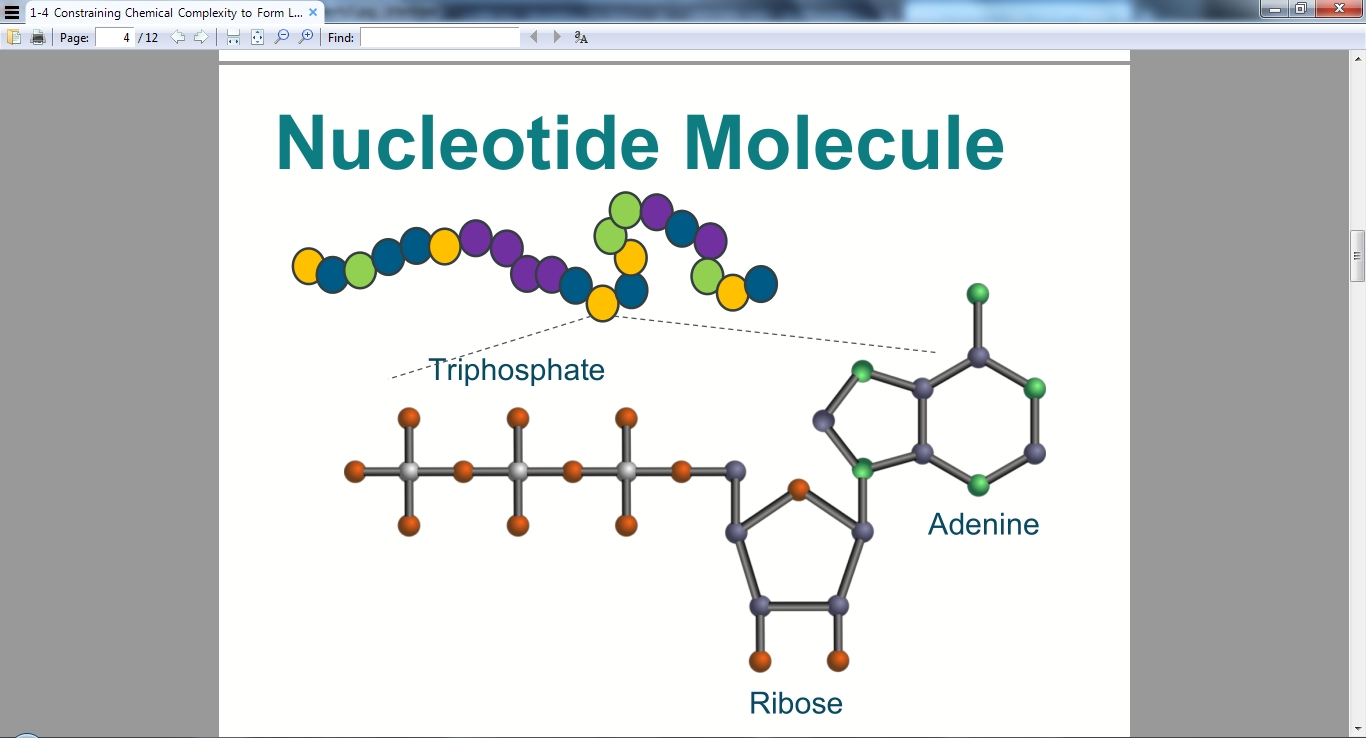
\includegraphics[width=\textwidth]{NucleotideMolecule}
	\end{subfigure}
	\begin{subfigure}[b]{0.45\textwidth}
		\centering
		\caption{Zoom into Adenine Molecule: change one thing, not adenine any more!}\label{fig:adenine}
		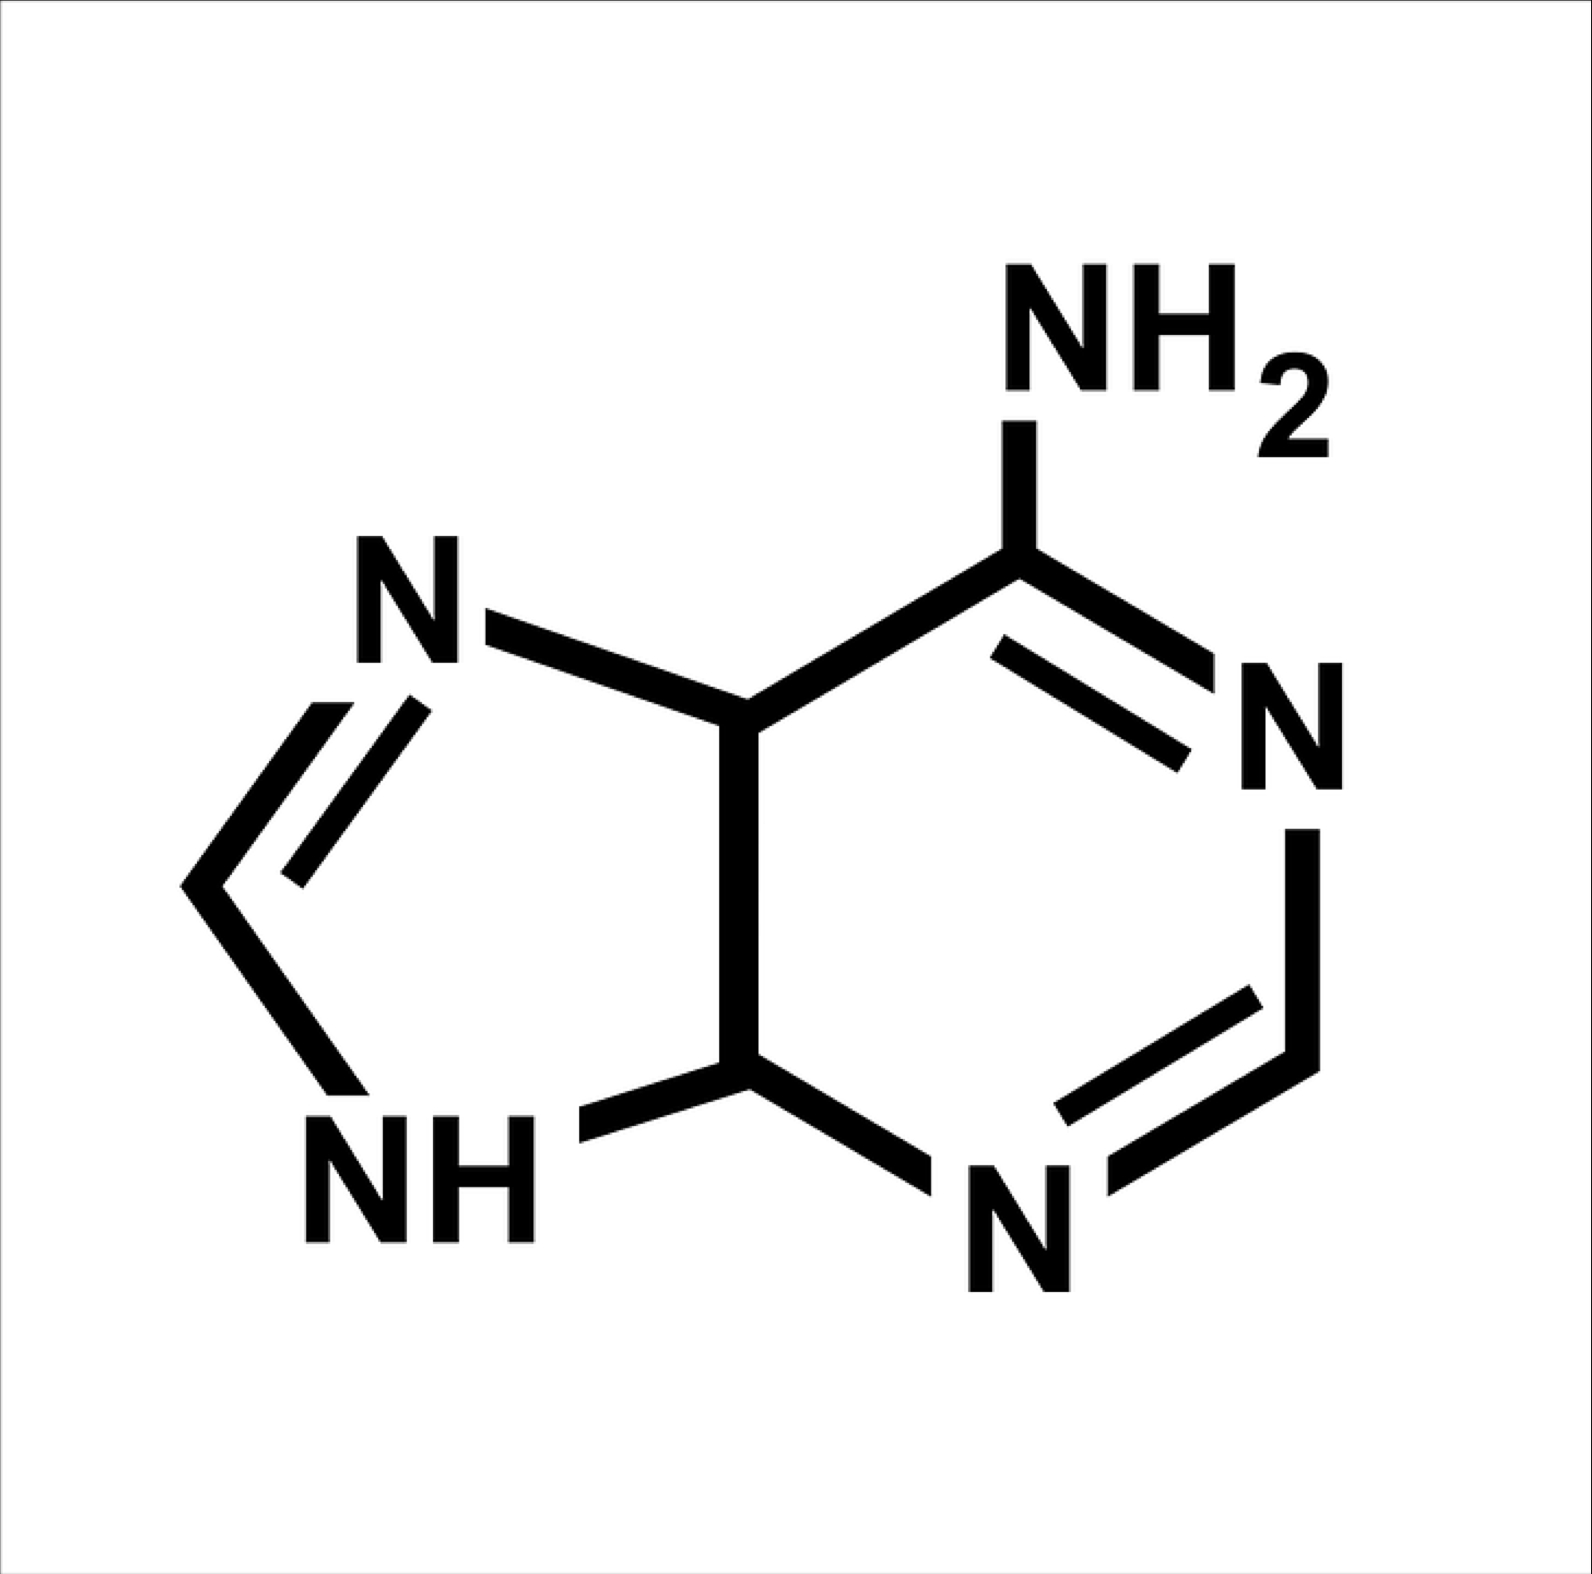
\includegraphics[width=0.6\textwidth]{AdenineMolecule}
	\end{subfigure}
\end{figure}

Let's zoom in further on the Adenine molecule, Figure \ref{fig:adenine}: change any atom and it wouldn't be adenine; now zoom in even further, Figure \ref{fig:MolecularInteractions}, and we see more interactions between atoms and with solvent.

\begin{figure}[H]
	\begin{center}
		\caption[Zoom in further, and atoms interact with each other]{Zoom in further, and atoms interact with each other, and with solvents!}\label{fig:MolecularInteractions} 
		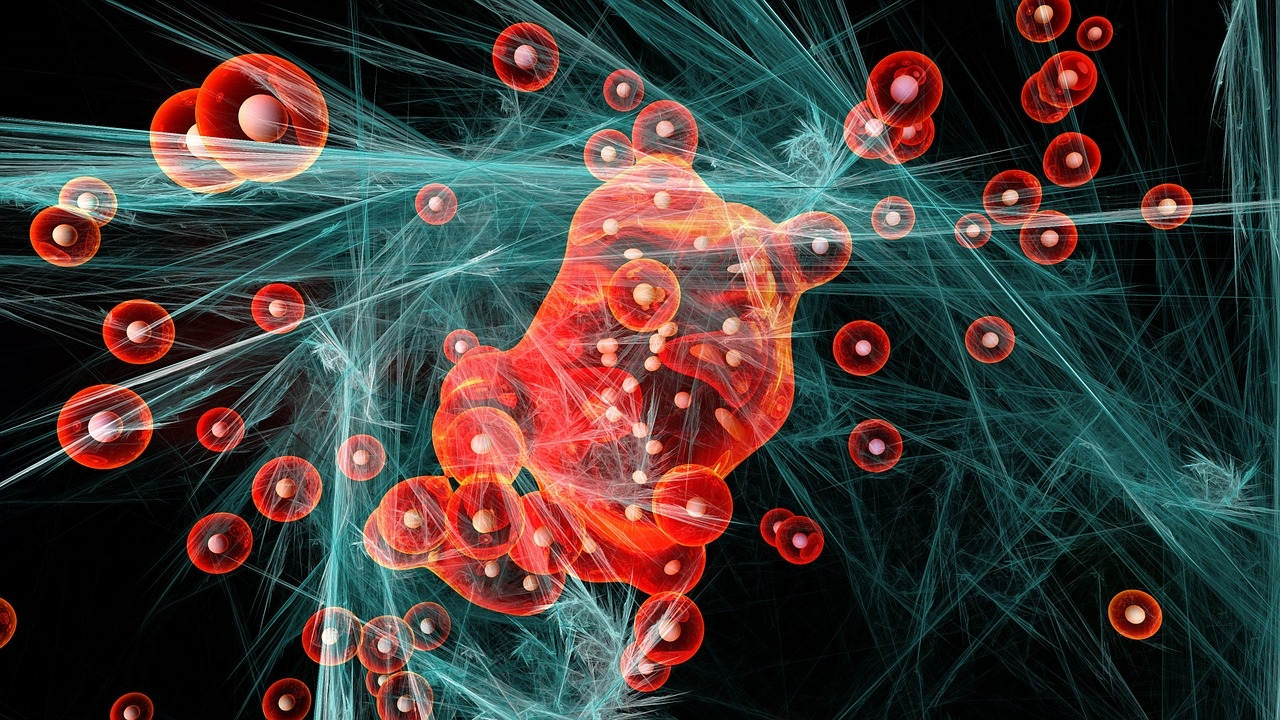
\includegraphics[width=0.9\textwidth]{MolecularInteractions}
	\end{center}
\end{figure}

If you want to think about generating these molecules from scratch, you need to think about all these interactions and their effects.

There are a number of ways origins of life researchers try to navigate this complexity and design experiments that get to the root of how life could have originated from a non-living state.

\begin{itemize}
	\item Constrain Location 
	\begin{itemize}
		\item Advantages
		\begin{itemize}
			\item Many possibilities for complex interactions
			\item Experiments can be designed by analogy with modern environments.
		\end{itemize}
		\item Disadvantages: mostly implausible to assume pure reactants in natural settings
	\end{itemize}
	\item Constrain Reactants
	\begin{itemize}
		\item Advantages: limit to needed molecules and needed amounts.
		\item Disadvantages: resulting network is not very complex or robust
	\end{itemize}	
	\item Constrain Energy Sources
		\begin{itemize}
		\item Advantages: processes are not location- or reactant-specific; many 		outcomes are possible
		\item Disadvantages: Difficult or impossible to predict outcomes of
		processes that cross multiple object levels
	\end{itemize}
\end{itemize}

Examples
\begin{itemize}
	\item Constrained Location Examples \begin{itemize}
		\item Hydrothermal Vents\cite{martin2006origin}
		\item Atmosphere (Impactor/Shock Synthesis, Lightning,
		Insolation)\cite{chyba1992endogenous} \cite{miller1959organic}
	\end{itemize}
	\item Constrained Reactant Examples 
	\begin{itemize}
		\item RNA World\cite{powner2009synthesis},
		\item Pyrite-mediated synthesis\cite{wachtershauser1993cradle}
		\item Borate-mediated synthesis\cite{grew2011borate}
	\end{itemize}
	\item Constrained Energy Examples
	\begin{itemize}
		\item \Gls{gls:serpentinization}\cite{schrenk2013serpentinization}
		\item Solar flares\cite{airapetian2016prebiotic}
		\item Radioactivity\cite{yi2018radiolytic} \cite{adam2018estimating}
	\end{itemize}
\end{itemize}

\section[Geological Conditions, Change, and Chaos]{Geological Conditions, Change, and Chaos--Zach Adam}

What is the source of our understanding of conditions when we thought life originated?
\begin{figure}[H]
	\caption[Earth's Structure]{Earth's Structure: includes everything in Figure, plus minerals, etc. We can only sample surface, plus a few km  down.}\label{fig:EarthStructure} 
	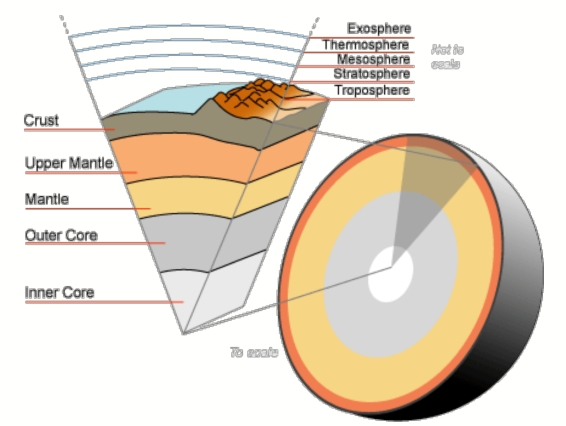
\includegraphics[width=0.9\textwidth]{EarthStructure}
\end{figure}

Continents don't stay in the one place. So what we say today may not be what was there in the past.
\begin{figure}[H]
	\caption{Geologic Record is inseparable from history of life}\label{fig:GeologicRecord} 
	
	\begin{subfigure}[b]{0.45\textwidth}
		\centering
		\caption{Great oxidation event changed all sorts of stuff. We need oxygen, but other critters had to adapt or die. Oxidation changed minerals.}
		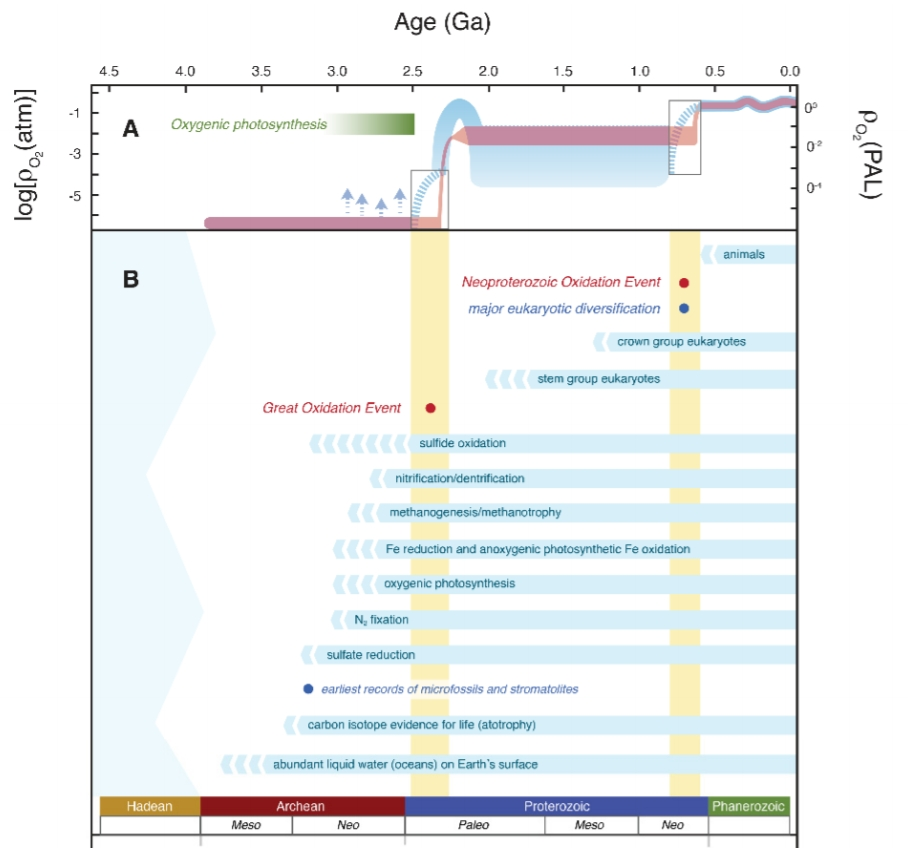
\includegraphics[width=0.8\textwidth]{GeologicRecord}
	\end{subfigure}
	\begin{subfigure}[b]{0.45\textwidth}
		\centering
		\caption{How much change has been caused by weathering? There are different models for crustal accumulation. So how much crust has been produced over time?}
		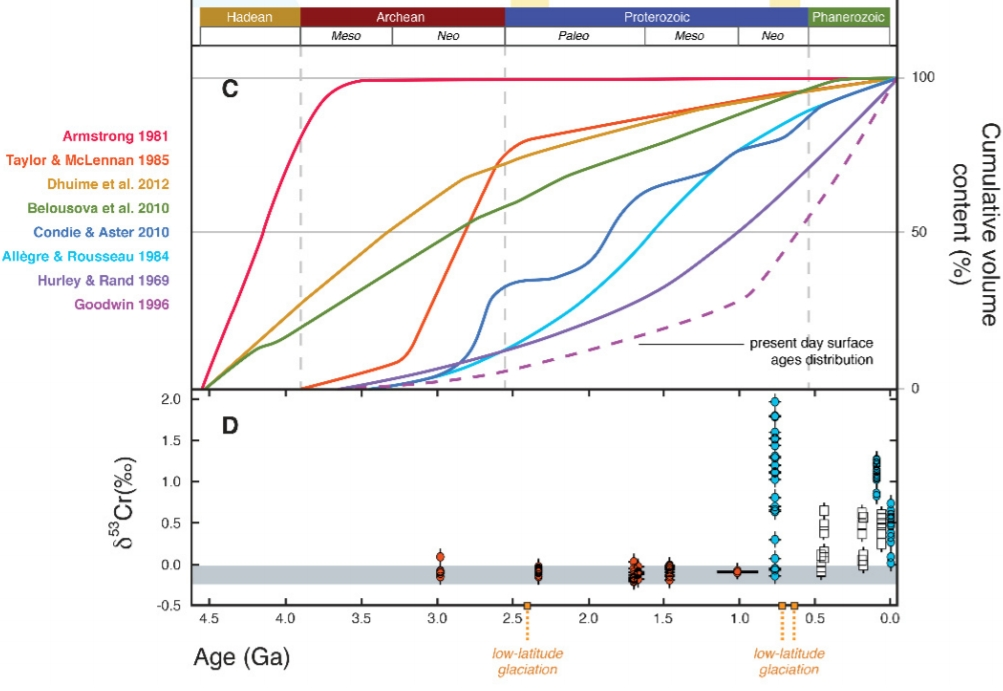
\includegraphics[width=\textwidth]{GeologicRecord1}
	\end{subfigure}
\end{figure}

\begin{figure}[H]
	\caption[Another Level Down: different models for accumulation of crust.]{Another Level Down: different models for accumulation of crust. Not simple accumulation! There may have been periods where there was more crust than today\cite{spencer2017growth}.}\label{fig:AnotherLevelDown} 
	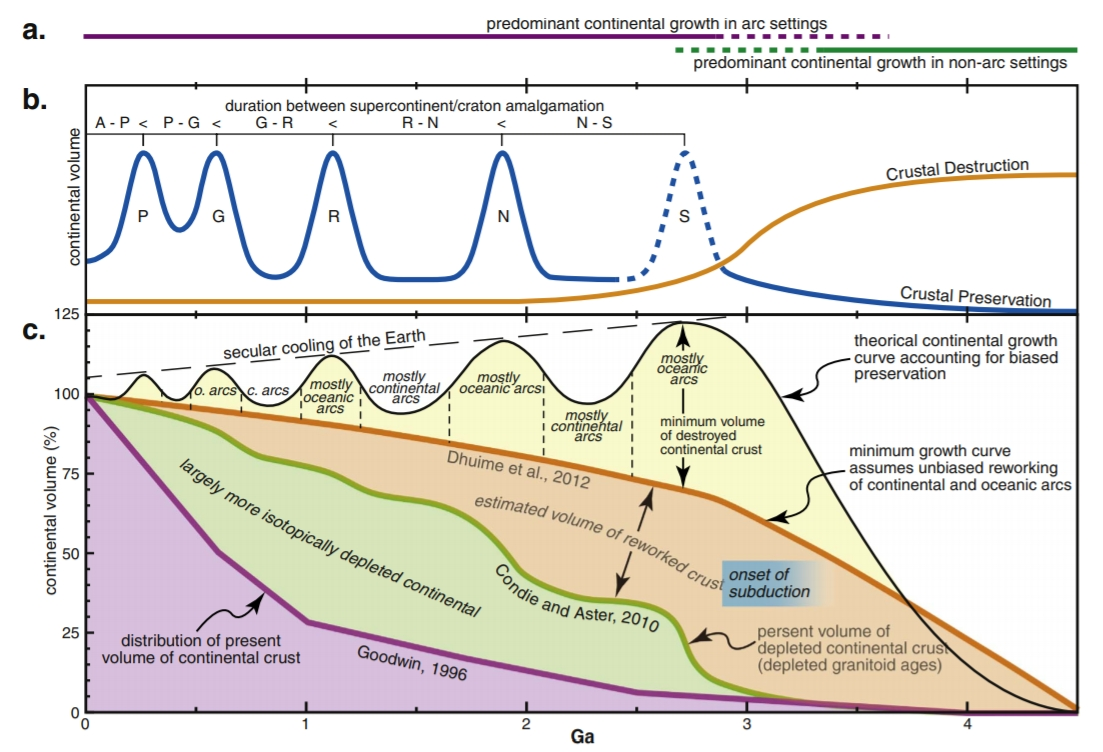
\includegraphics[width=0.9\textwidth]{AnotherLevelDown}
\end{figure}

Only direct record for events that sow chaos and processes of prolonged gradual change; much of the evidence for such events may have been lost.

What does this mean for origins of life research?
\begin{itemize}
	\item Limited direct rock data
	\begin{itemize}
		\item 	Sampling and preservation
		biases abound!
			\item No rock packages to
		provide environmental
		context or views into surface
		conditions.
		\item 	No rocks and few minerals
		from time surrounding life’s
		origins.
	\end{itemize}
	\item Complementary lab data
	\begin{itemize}
		\item Experiments are critical for
		filling in where the rock
		record is not available.
			\item Unclear whether powerful
		events/energy are more
		constructive than destructive.
	\end{itemize}
\end{itemize}

\section[Pattern Formation in Chemical Systems]{Pattern Formation in Chemical Systems-- Chris Kempes}

\begin{itemize}
	\item What properties and processes are easy to obtain through physical dynamics alone?	
	\item How might this make it easy for lifelike things to begin?
\end{itemize}

We will look at pattern formation through the lens of Reaction Diffusion Equations\cite{sfi_grayscott2018}.

Here is a very simple reaction diffusion equation. It relates the change in concentration of some chemical,  $U$, to a diffusion plus a reaction.
\begin{align*}
\frac{\partial U}{\partial t} =&   \underbrace{\overbrace{D_V}^\text{diffusivity} \underbrace{ \nabla^2 U }_\text{difference in fluxes}}_\text{diffusion term} + \underbrace{ F(U)}_\text{reaction term}
\end{align*}

With two chemicals...
\begin{align*}
\frac{\partial U}{\partial t} =&   D_U \nabla^2 U + F(U,V)\\
\frac{\partial V}{\partial t} =&   D_V \nabla^2 V + G(U,V)
\end{align*}

Now let's consider a specific example.
Consider two reacting species, $U$ and $V$, and an inert product $P$.
\begin{align*}
U + 2V \Longrightarrow& 3V\\
V \Longrightarrow& P
\end{align*}

\begin{enumerate}
	\item The first term in (\ref{eq:U}) represents the reaction of $U$ with $2V$. 
	\item We have chemostated the system, meaning there is some constant flux into the system and out of the system. $F(1 - U)$ represents flow in and out.
	\item Middle term in (\ref{eq:V}) represents outflow of $V$ plus conversion to $P$.
\end{enumerate}
\begin{align*}
	\frac{\partial U}{\partial t} =& -U V^2 + F(1 - U)  + D_u \nabla^2 U \numberthis \label{eq:U}\\
	\frac{\partial V}{\partial t} =& U V^2 - (F +k) V + D_v \nabla^2 V \numberthis \label{eq:V}
\end{align*}

This set of equations gives rise to very interesting spatial patterns. Using stability analysis we can determine the range of $F$ and $k$ that allow interesting patterns to form--Figure \ref{fig:GreyScottRange}.

\begin{figure}[H]
	\caption{Grey Scott Reaction}
	\begin{subfigure}[b]{0.3\textwidth}
		\centering
		\caption{the range of $F$ and $k$ that allow interesting patterns to form.}\label{fig:GreyScottRange}
		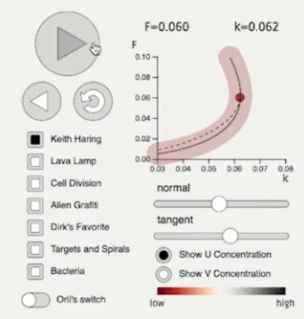
\includegraphics[width=\textwidth]{GreyScottRange}
	\end{subfigure}
	\begin{subfigure}[b]{0.3\textwidth}
		\centering
		\caption{Starting configuration}
		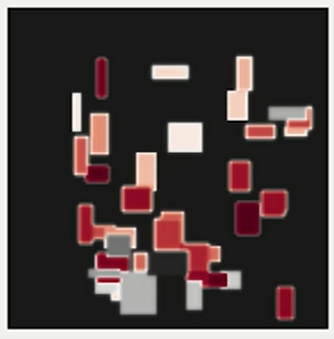
\includegraphics[width=\textwidth]{GreyScottInitial}
	\end{subfigure}
	\begin{subfigure}[b]{0.3\textwidth}
		\centering
		\caption{Evolves toward steady state,  where high concentration close to low concentration.}
		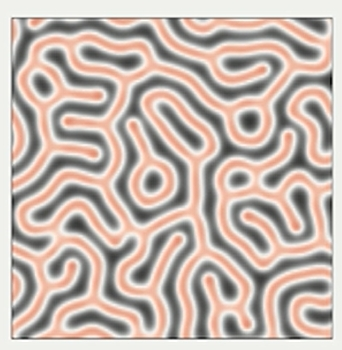
\includegraphics[width=\textwidth]{GreyScottFinal}
	\end{subfigure}
\end{figure}

What is very nice about this is it tells us that in a very simple context where we are combining this reaction with diffusion we see this very interesting pattern formation with strong spacial gradients: very high concentrations of $U$ and $V$ are separated by small distances and we see segregation. We can get very different concentrations very close to one another. This gives us hope, from an origins of life point of view, of getting complicated chemistry forming close to other complicated chemistry on small spatial scales in a way that is stable and segregated. 

Other starting values give cell-like behaviour (including division), so maybe get some ''lifelike" behaviour from physics and simple chemistry.

\section[The Central Dogma of Biology]{The Central Dogma of Biology--Chris Kempes}


\subsection{The Central Dogma of Biology}

One of the overarching questions of this class is how do we unwind present day life to learn about origins? Focus on most common properties of all life, especially the Central Dogma.\cite{crick1958biological} \cite{crick1970central}

\begin{figure}[H]
	\caption[The Central Dogma]{The Central Dogma after \cite{crick1970central}}\label{fig:CentralDogma} 
	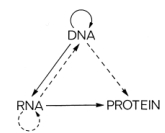
\includegraphics[width=0.9\textwidth]{CentralDogma}
\end{figure}


\begin{figure}[H]
	\caption[Ribosome is conserved across life]{Ribosome is conserved across life, but appears to have onion structure, built up by evolution. Ribosome started with common core, and more added.\cite{hsiao2009peeling}.}\label{fig:Ribosome} 
	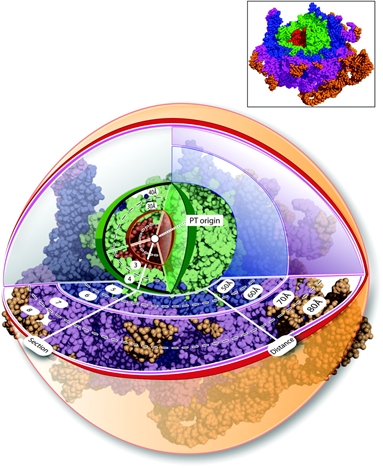
\includegraphics[width=0.9\textwidth]{Ribosome}
\end{figure}
Williams argues that we can use the onion, Figures \ref{fig:Ribosome} and \ref{fig:RibosomePhases}, to unwind evolution.

\begin{figure}[H]
	\caption[Ribosome Phases]{Ribosome Phases after \cite{petrov2015history}, illustrating evolution of  \gls{gls:LSU} and \gls{gls:SSU}}\label{fig:RibosomePhases} 
	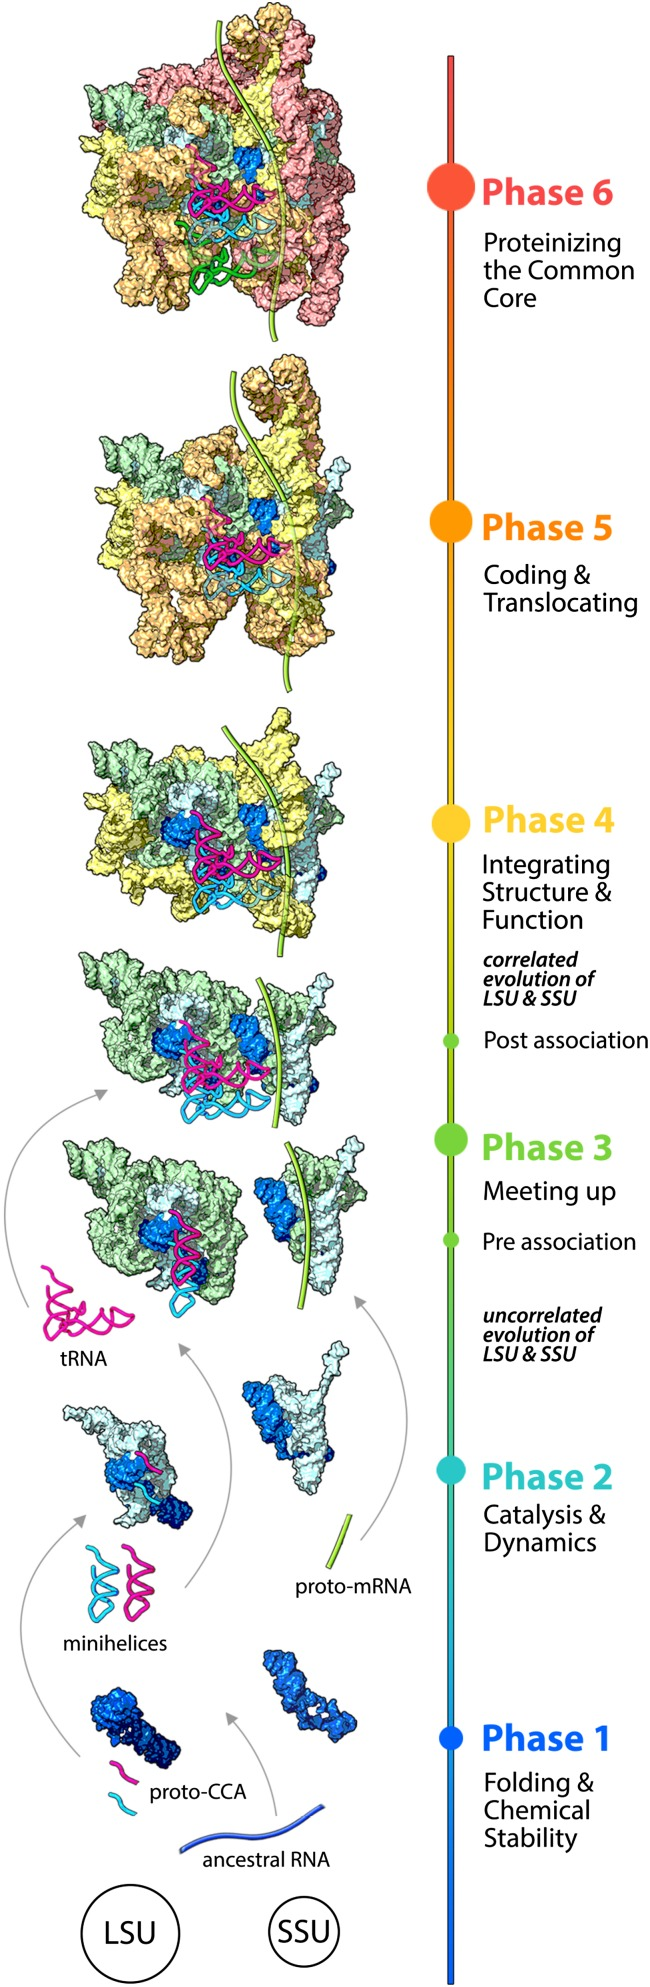
\includegraphics[width=0.5\textwidth]{RibosomePhases}
\end{figure}

Carl Woese used this to build new a Tree of Life.

\begin{figure}[H]
	\caption[Tree of Life]{\gls{gls:TOL}\cite{nair2012woese}}\label{fig:TOL} 
	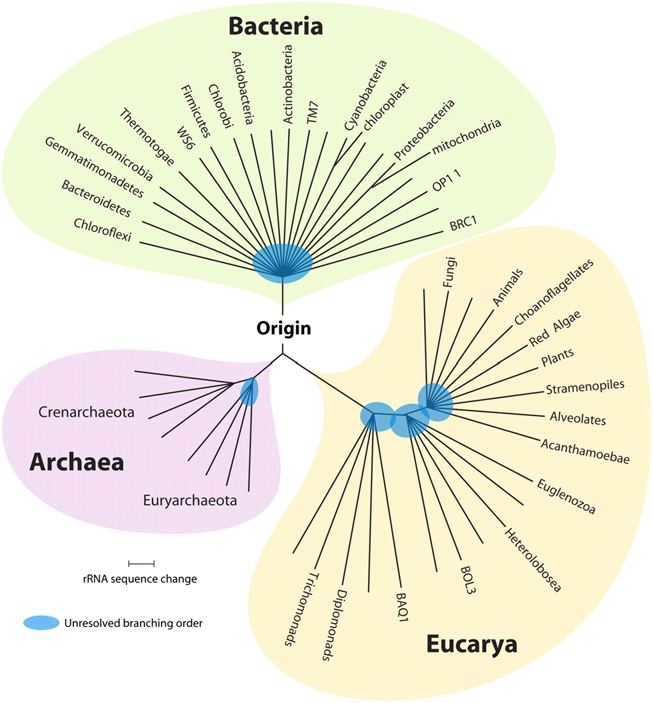
\includegraphics[width=0.9\textwidth]{TOL}
\end{figure}

\subsection{The Efficiency of the Central Dogma of Biology}

\gls{gls:landauer_bound}: \glsdesc{gls:landauer_bound}. 

\begin{figure}[H]
	\caption[Take unordered set of letters and try to write as specific string]{Take unordered set of letters and try to write as specific string\cite{kempes2017thermodynamic}}\label{fig:LandauerRibosome} 
	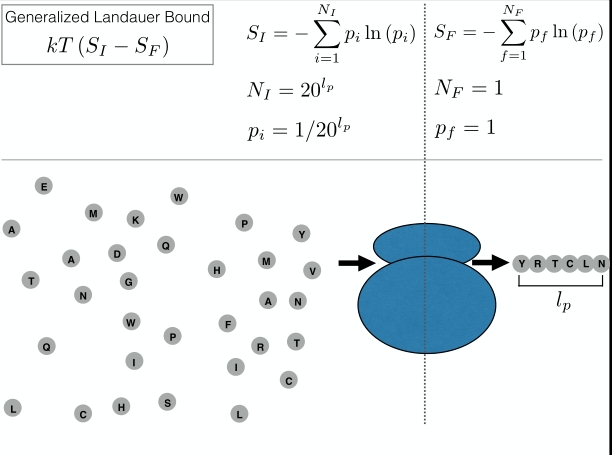
\includegraphics[width=0.9\textwidth]{LandauerRibosome}
\end{figure}

\begin{itemize}
	\item Life is only 20 times less efficient that physical limit\cite{kempes2017thermodynamic}
	\item Computers are 100,000,000 times worse than Landauer's bound!
\end{itemize}

\begin{figure}[H]
	\caption{Ribosome Tradeoffs}
	\begin{subfigure}[b]{0.45\textwidth}
		\caption{For a small cell, DNA and proteins take up (nearly) entire volume; for large cells, Ribosome does same thing! So we have bounds on allowable volume.\cite{kempes2016evolutionary}}\label{fig:RibosomeTradeoffs} 
		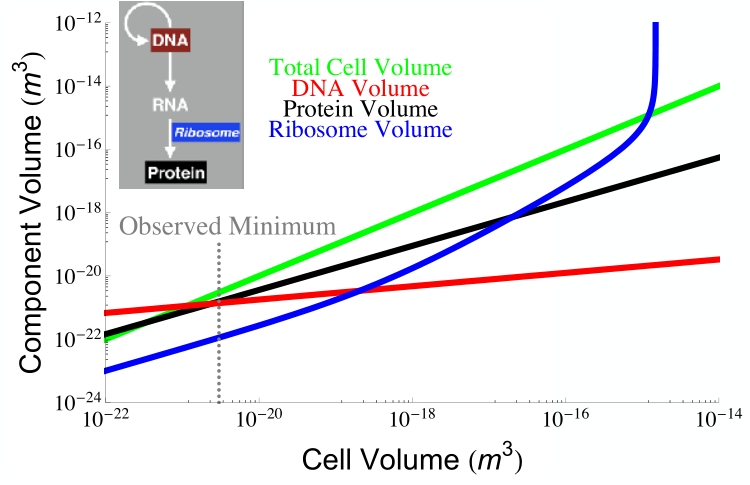
\includegraphics[width=\textwidth]{RibosomeTradeoffs}
	\end{subfigure}
	\;\;\;
	\begin{subfigure}[b]{0.45\textwidth}
		\caption{A more efficient ribosome would allow larger cells; less efficient might not work at all.}\label{fig:RibosomeTradeoffsEarly} 
		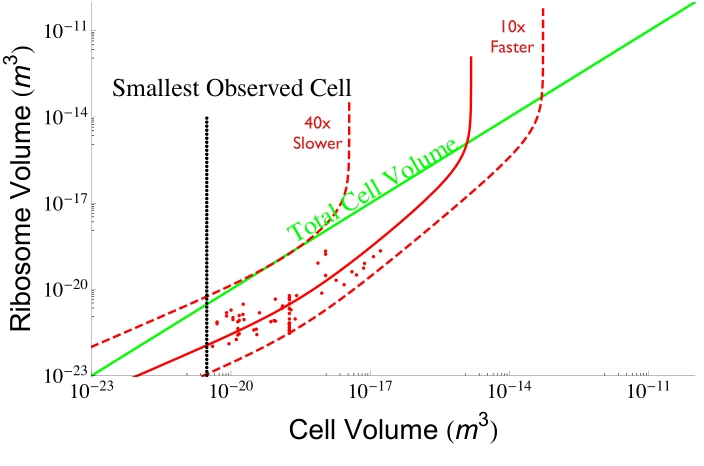
\includegraphics[width=\textwidth]{RibosomeTradeoffsEarly}
	\end{subfigure}
\end{figure}
\section[Biological Similarity]{Biological Similarity--Sarah Mauer}

We will use a top-down approach.

 ''By examining and deconstructing the commonalities between modern living organisms, we can better understand the requirements of first life.''

\begin{itemize}
	\item \Gls{gls:chirality}--Figure \ref{fig:Chirality}
	\begin{itemize}
		\item L-amino acids for all proteins;
		\item D-sugars for all sugars and nucleic acids.
	\end{itemize}
	\item The next thing that all living organisms have in common
	is that they use membranes to separate themselves from the environment--Figure \ref{fig:Membranes}--and these membranes are composed of amphiphilic molecules which have two parts:  a hydrophobic tail that aggregates between itself and a hydrophilic head group that interact with the water phase. This creates a barrier to the environment and also helps to keep important molecules inside the cell.
	Many/membranes are used to separate cells from one another they are also used
	to separate \glspl{gls:organelle} from other parts of the cell;
	one organelle is the nuclear membrane which separates the nucleic acid from the \gls{gls:cytosol}.
	\item The nucleic acids are another component that all living things have in common. The small chemical structures that you see here are very highly conserved between all nucleic acids. DNA similarities:\begin{itemize}
		\item little difference in chemical structure between organisms
		\item some difference in packing
		\item large difference in the size of genome
	\end{itemize}
	\item All cells use proteins, made from the same 20 amino acids.
\end{itemize}

\begin{figure}[H]
	\caption[L-amino acids and D-sugars]{L-amino acids for all proteins; D-sugars for all sugars and nucleic acids}\label{fig:Chirality}
	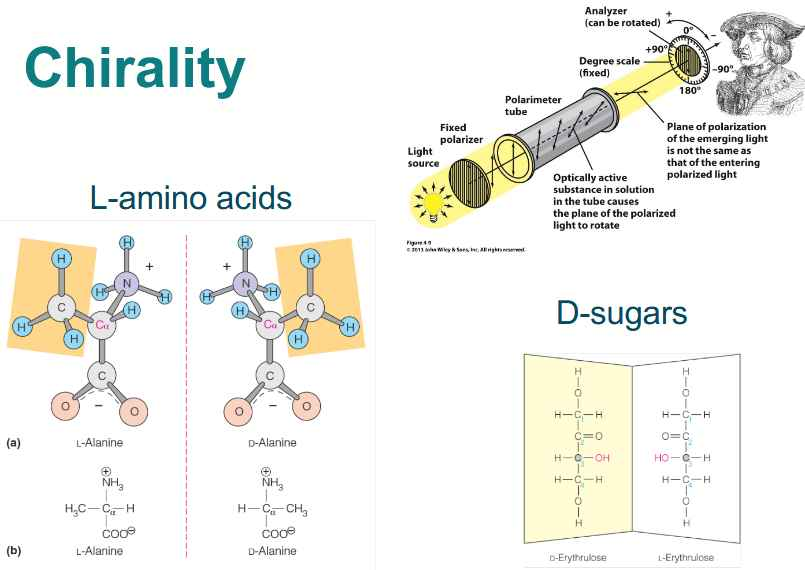
\includegraphics[width=0.8\textwidth]{Chirality}
\end{figure}

\begin{figure}[H]
	\caption[All living organisms use membranes]{All living organisms use membranes to separate themselves from the environment}\label{fig:Membranes}
	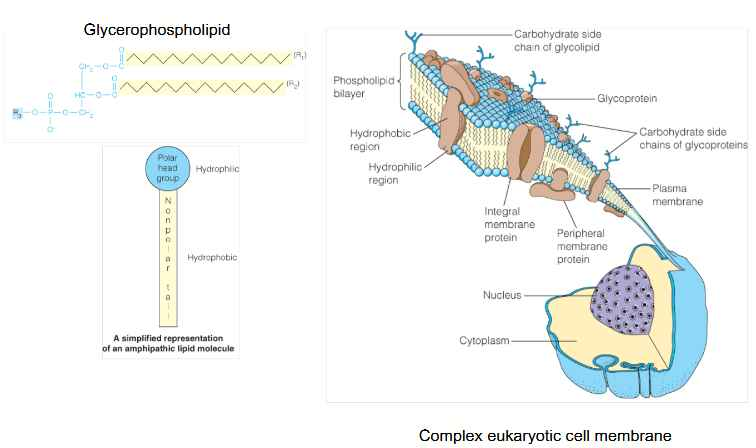
\includegraphics[width=0.8\textwidth]{Membranes}
\end{figure}
\begin{figure}[H]
	\caption[Comparison of similarity allows for the
		construction of a tree]{Comparison of similarity allows for the
		construction of a tree, outlining evolution. Large part of conserved set involved in Central Dogma, and also metabolic.}\label{fig:Phylogeny} 
	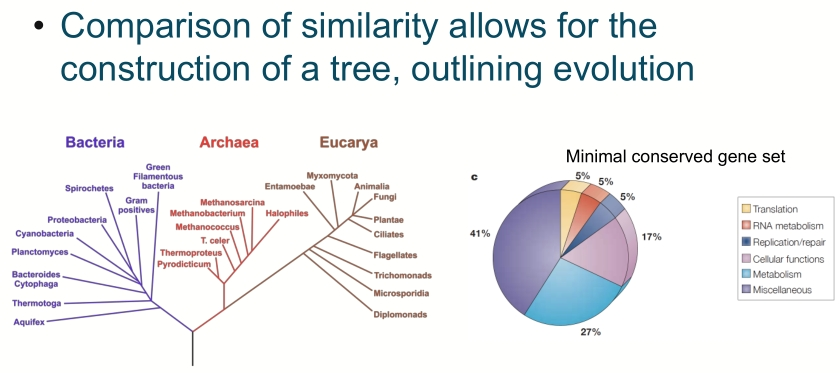
\includegraphics[width=0.9\textwidth]{Phylogeny}
\end{figure}

\begin{figure}[H]
	\caption{Horizontal gene transfer complicates things!}\label{fig:PhylogenyHorizontal} 
	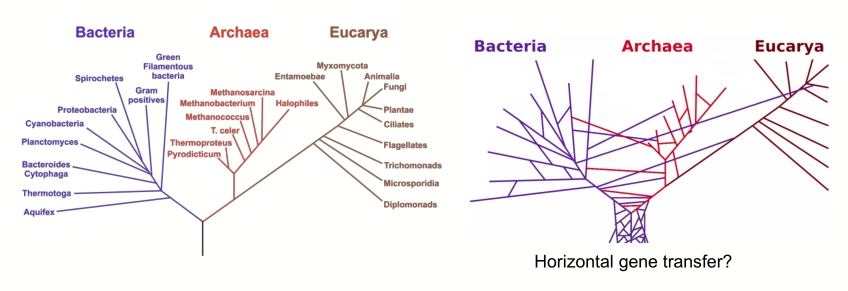
\includegraphics[width=0.9\textwidth]{PhylogenyHorizontal}
\end{figure}



\section{What is Life?}

\subsection[Constraining the Definition of Life]{Constraining the Definition of Life--Sara Imari Walker}

Schrödinger wondered whether we could explain life using physics as currently known.

''... living matter, while not eluding the laws of physics as established up to date, is likely to involve other laws of physics hitherto unknown''--Erwin Schrödinger\cite{schrodinger1944life}.

WE don't really know what life looks like, but we might ask critically what are the examples of life on Earth, and how we can use them to build a unified theory of what life is--a real predictive theory that allows us to understand nit just life on this planet, but also life on other worlds. In physics we have this wonderful hierarchy of theories--Figure \ref{fig:physics:unifications}, but it doesn't have anything to say about complex systems or about us: ''The theory of everything is a theory of everything except of those things that theorize''--David Krakauer.

So the challenge is how can we think about how we can approach an explanatory theory for life, and whether we can draw inspiration from the history of physics. So it is constructive to look at examples of life on earth. Is life really a natural kind? Are some systems more alive than others?

\begin{figure}[H]
	\caption{History of Unifications in Physics}
	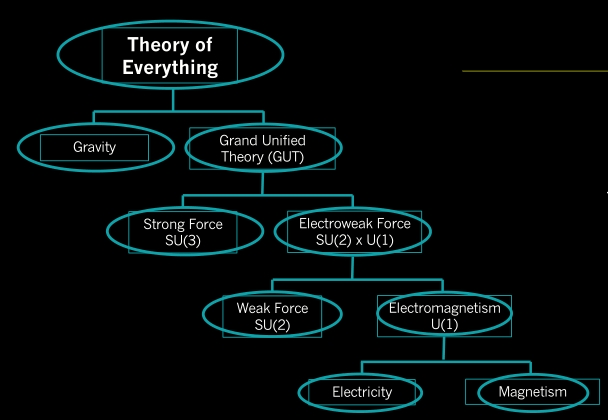
\includegraphics[width=0.9\textwidth]{Unifications}\label{fig:physics:unifications}
\end{figure}


Examples of "Life"
\begin{itemize}
	\item The Cell as a unit of Life--Figure \ref{fig:cell}
	\item Metabolism--Figure \ref{fig:metabolism}
	\item Tardigrade--an extremophile that can live in space--Figure \ref{fig:tardigrade}. Maybe we should think about the widest set of conditions under which life \textit{can} exist.
	\item Two-headed planarian worms--Figure \ref{fig:2headed:planaria}. What is the limit for viable life?\cite{levin2019planarian}
	\item What if we replace RNA/DNA with XNA?
	\item We can consider scales of organization, as with Social Insects--Figure \ref{fig:social:insects}. Is the super-organism, the colony, "alive"? Is life something that emerges in chemistry, but can exist at higher levels?\cite{pratt2015psychology}
	\item Is a City alive--Figure \ref{fig:city}?
	\item Is there life on the scale of the Planet\cite{lovelock1974atmospheric}--Figure \ref{fig:gaia}?
\end{itemize}

\begin{figure}[H]
	\caption{The Cell as a unit of Life}\label{fig:cell}
	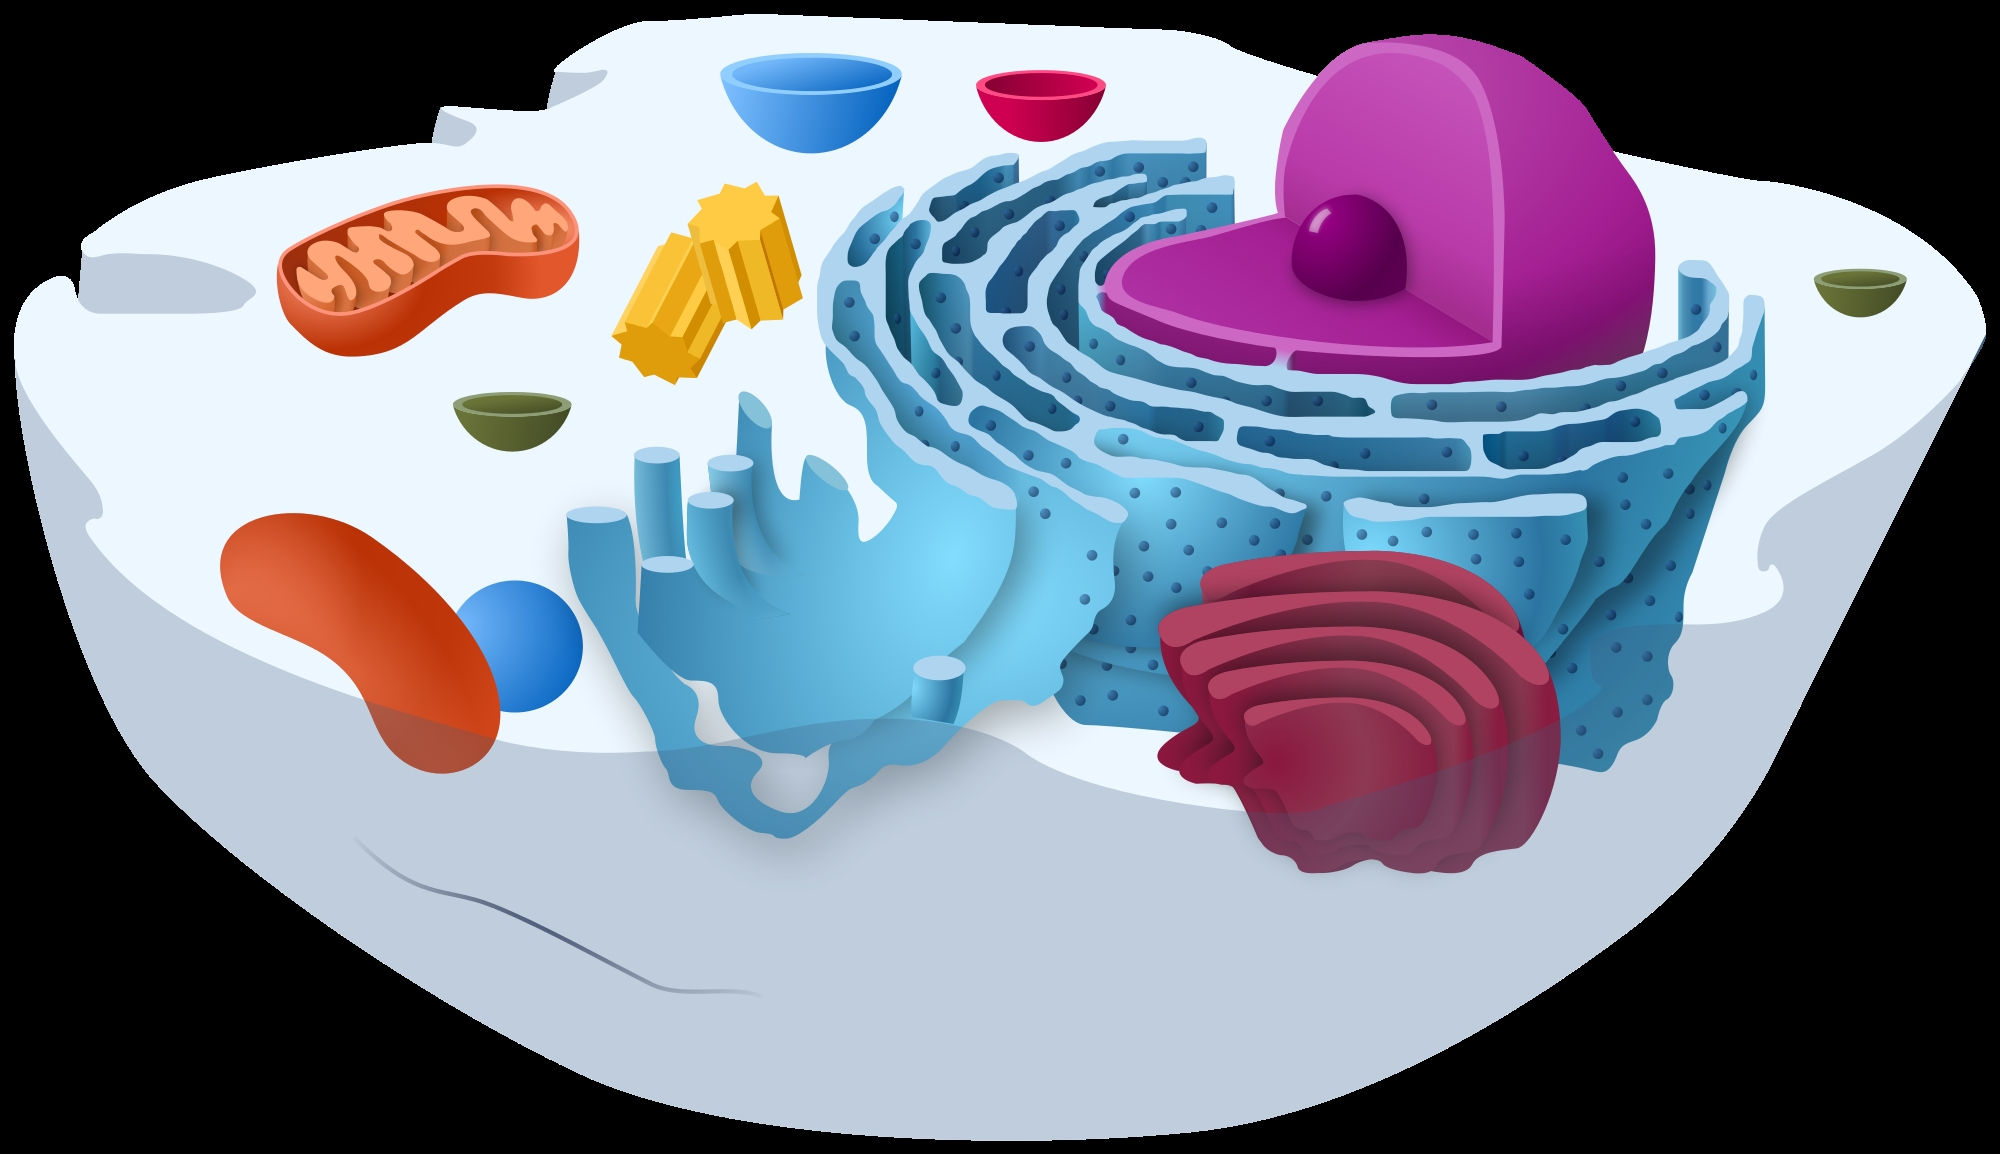
\includegraphics[width=0.9\textwidth]{Cell}
\end{figure}

\begin{figure}[H]
	\caption{Metabolism}\label{fig:metabolism}
	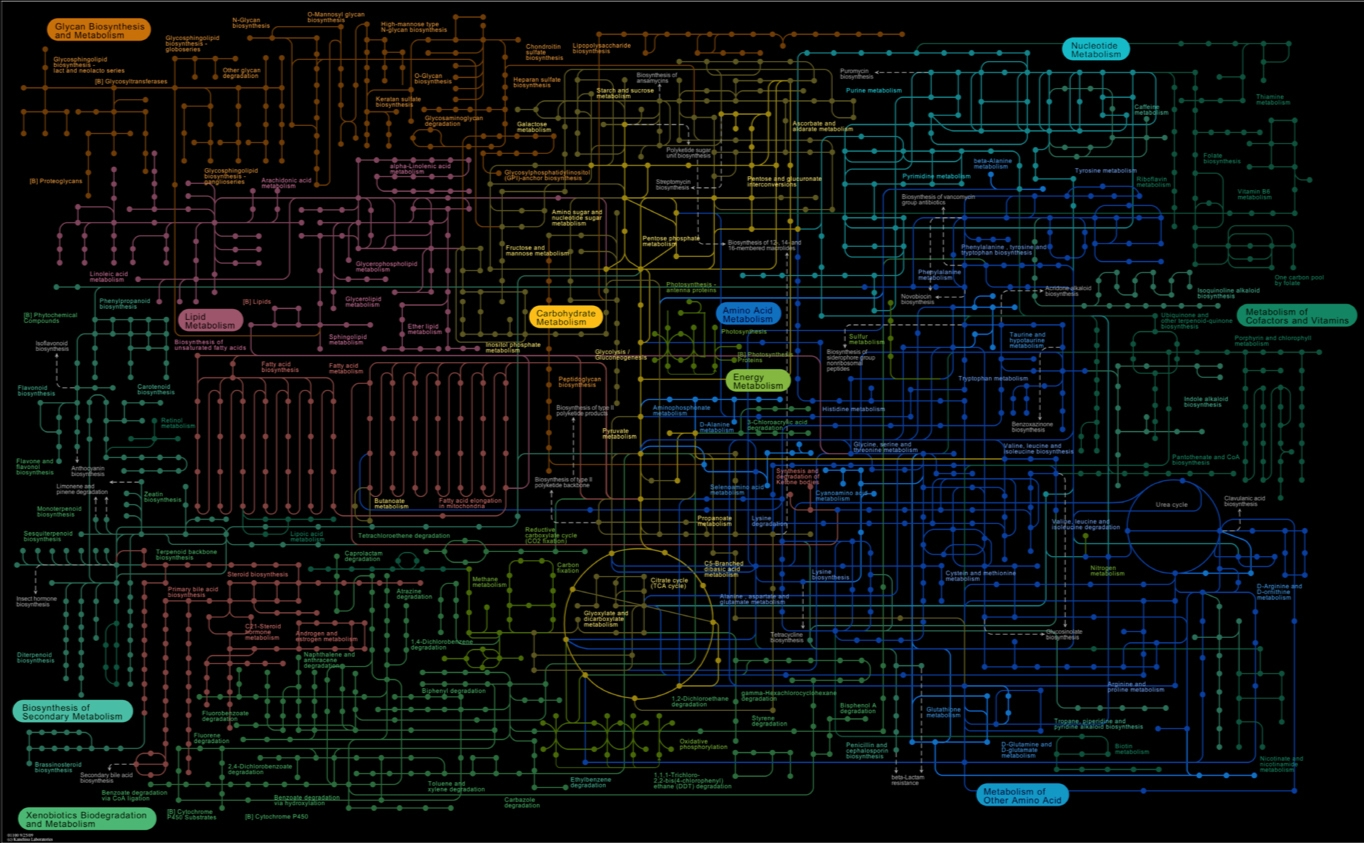
\includegraphics[width=0.9\textwidth]{Metabolism}
\end{figure}

\begin{figure}[H]
	\caption{Tardigrade--an extremophile that can live in space}\label{fig:tardigrade}
	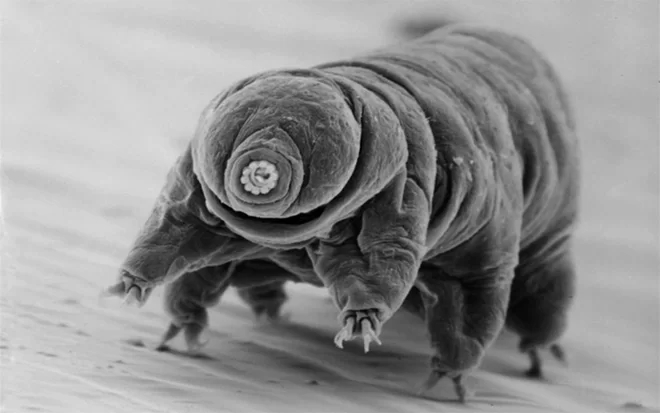
\includegraphics[width=0.9\textwidth]{Tardigrade}
\end{figure}


\begin{figure}[H]
	\caption{Two Headed Planaria}\label{fig:2headed:planaria}
	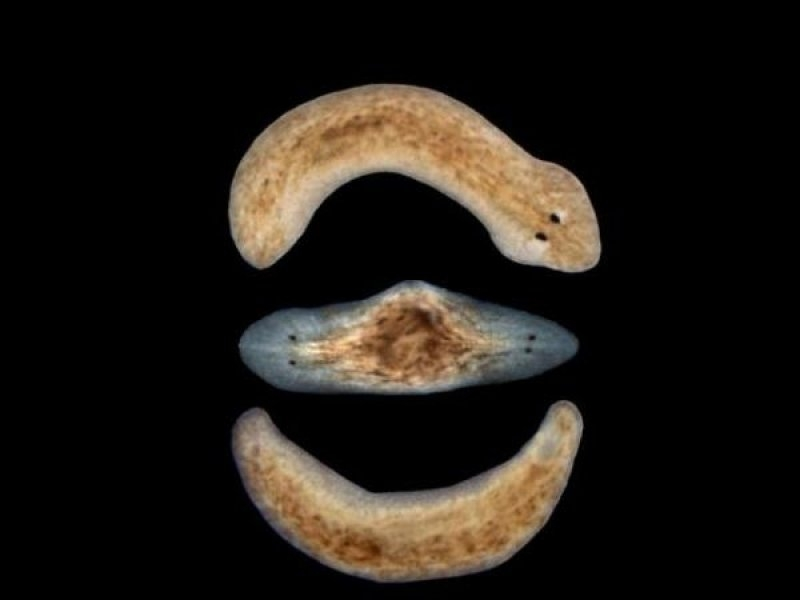
\includegraphics[width=0.9\textwidth]{TwoHeadedPlanaria}
\end{figure}

\begin{figure}[H]
	\caption{Social Insects: is the super-organism "alive"?}\label{fig:social:insects}
	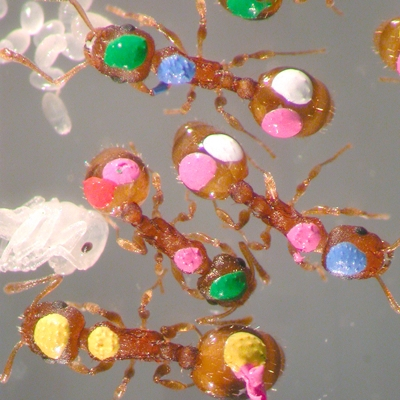
\includegraphics[width=0.9\textwidth]{SocialInsects}
\end{figure}

\begin{figure}[H]
	\caption{City}\label{fig:city}
	
\includegraphics[width=0.9\textwidth]{City}
\end{figure}

\begin{figure}[H]
	\caption{Is there Life on the scale of a Planet?}\label{fig:gaia}
	\begin{subfigure}[b]{0.45\textwidth}
		\caption{Gaia}
		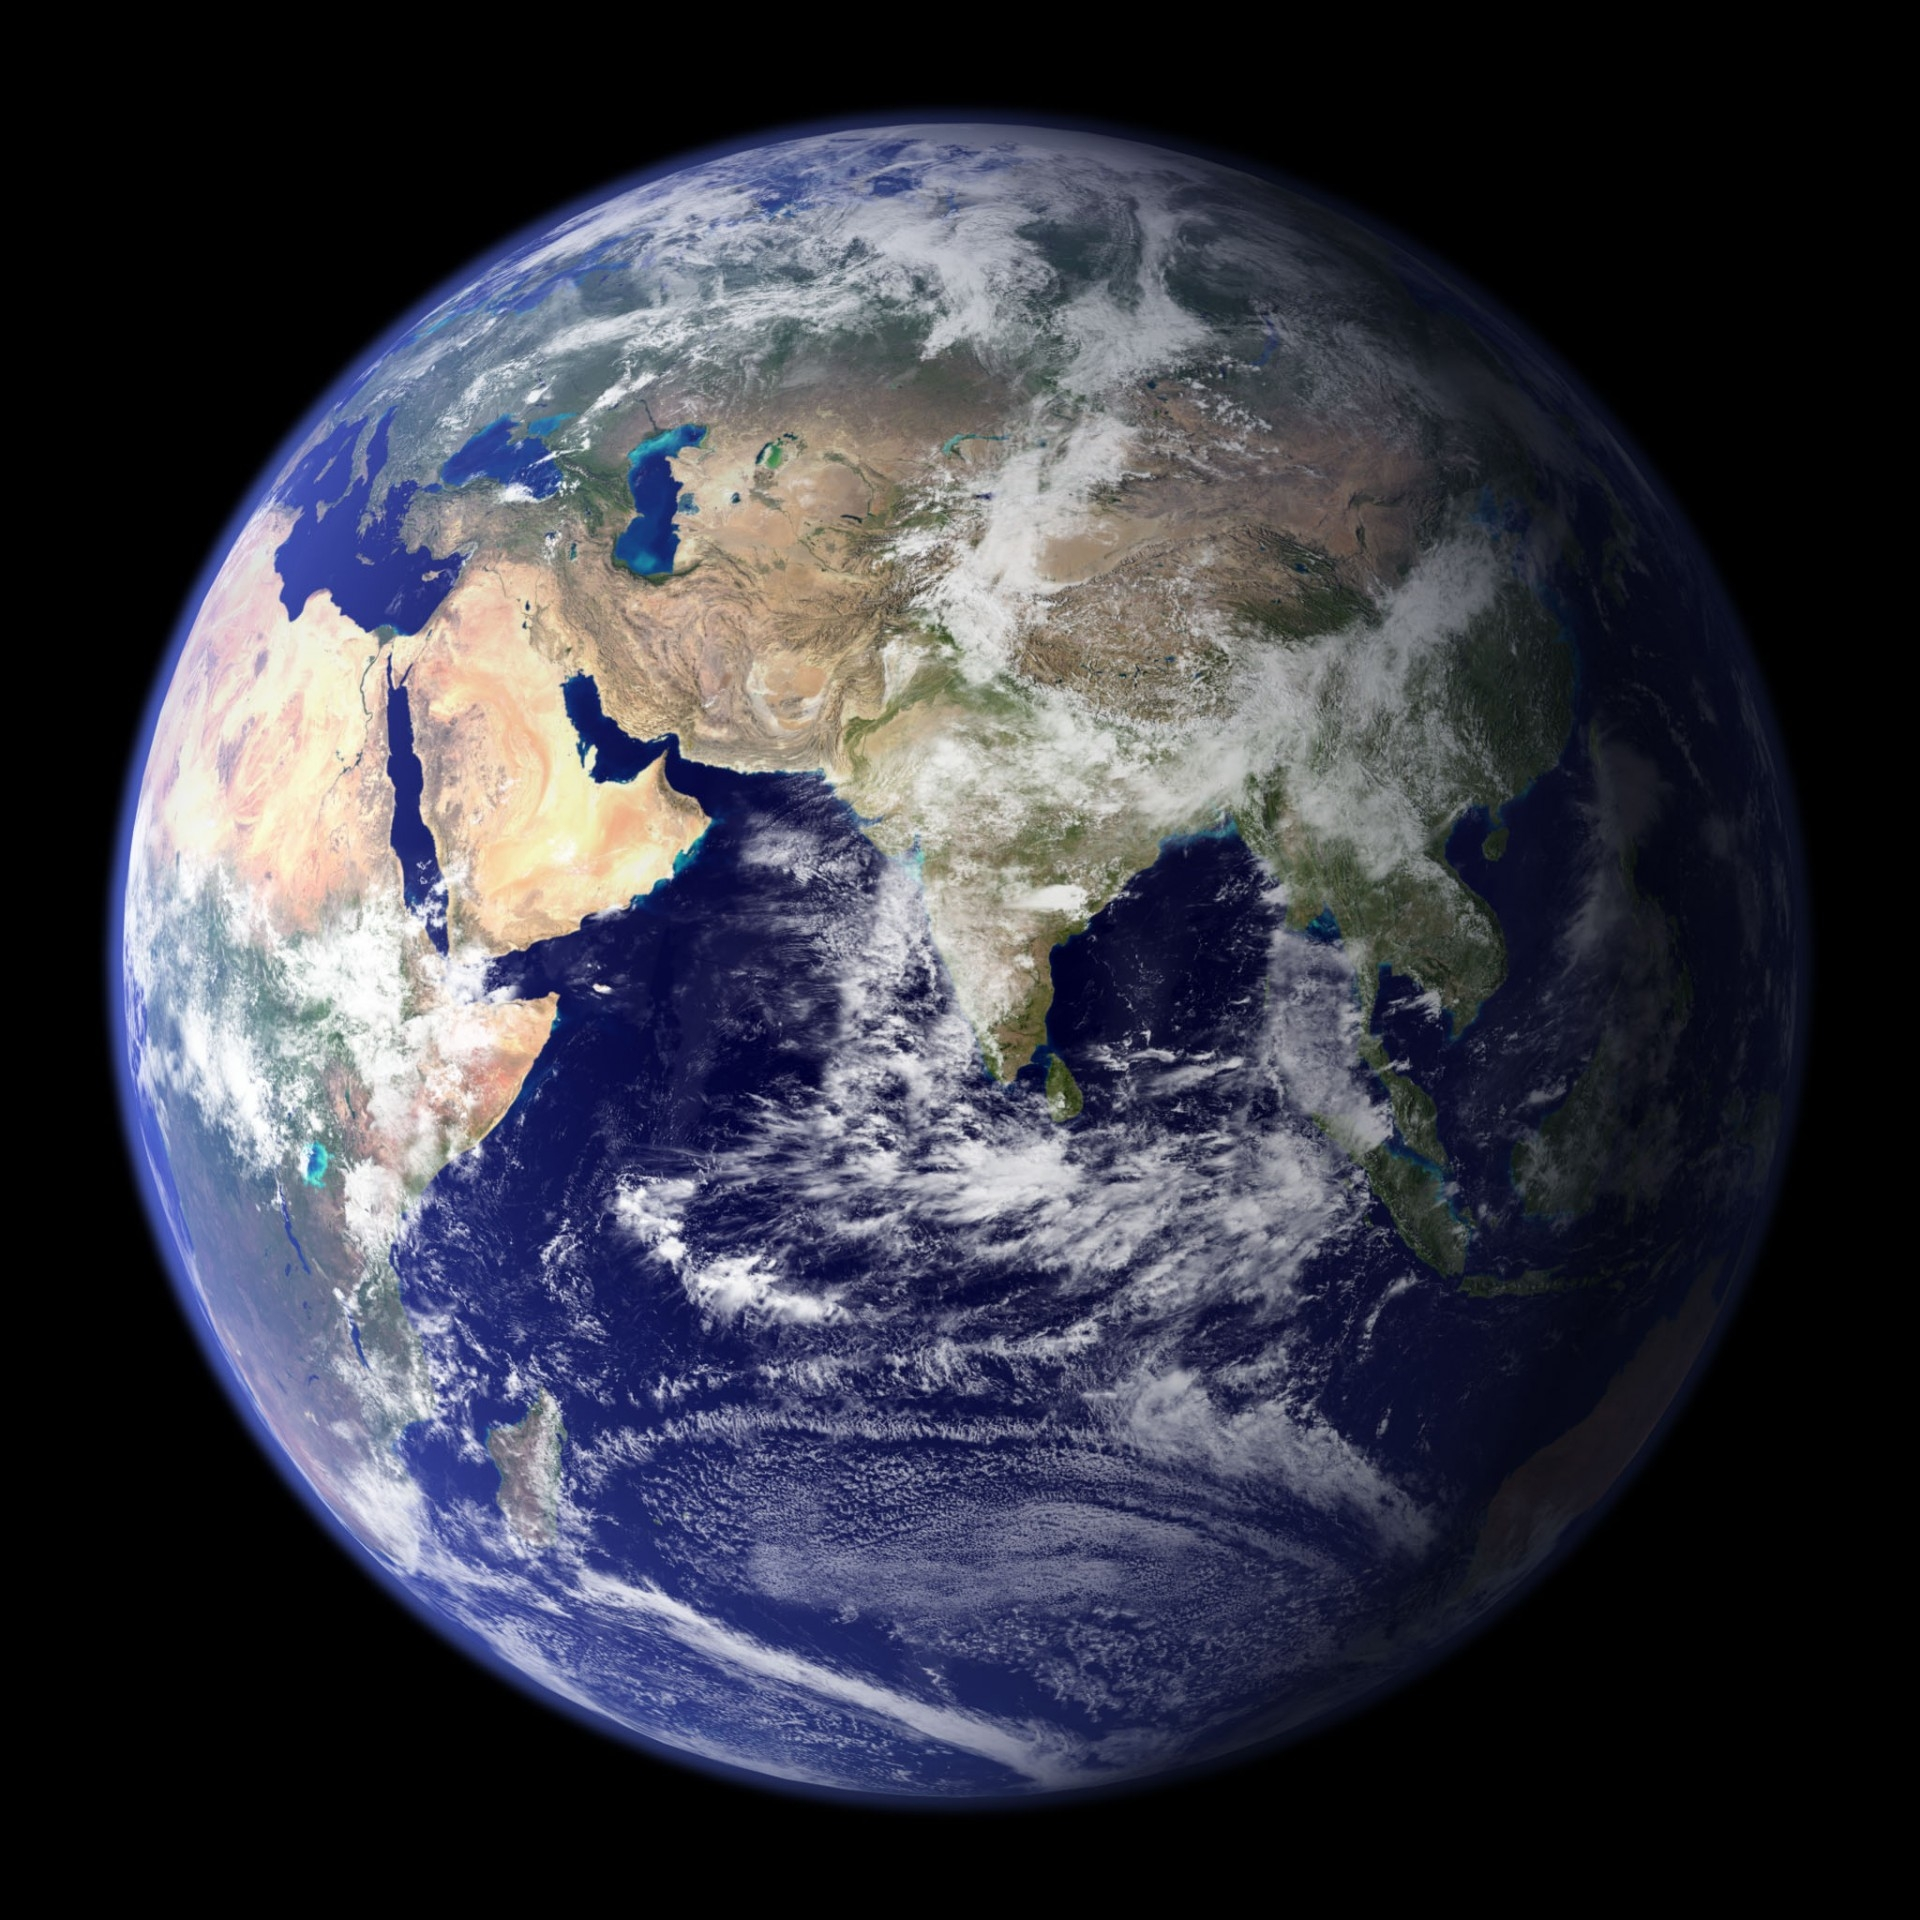
\includegraphics[width=\textwidth]{Globe1}
	\end{subfigure}
	\begin{subfigure}[b]{0.45\textwidth}
		\caption{Network representation of the global inventory of
			enzymatically catalyzed biochemical reactions}
		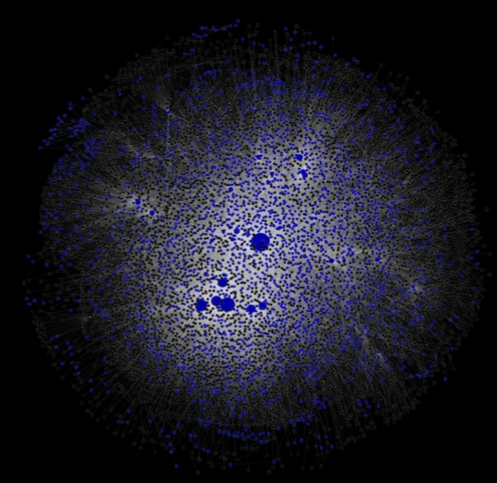
\includegraphics[width=\textwidth]{Globe2}
	\end{subfigure}
\end{figure}


\subsection[Weird Life]{Weird Life--Sarah Maurer}

The material in this section is entirely speculative.

\begin{itemize}
	\item No Cells--diffusion systems. But it is very restrained: have to get the right values for parameters.
	\item Membrane-less Cells? Organization of 	chemical gradients\cite{hollants2011life}\cite{kim2001life}
	\begin{itemize}
		\item Mineral surfaces
		\item Coacervates
		\item Oil droplets
		\item Aerosols
	\end{itemize}
	\item No water? 
	\begin{itemize}
		\item Polar solvents\cite[Chapter 6]{board2007limits}--Figure \ref{fig:no:water}. Water, ammonia, and sulphuric acid can:
		\begin{itemize}
			\item drive formation of carbon-carbon bonds;
			\item hydrogen bond.
		\end{itemize}
		\item Non-polar solvents\cite{cejkova2014dynamics}--Figure \ref{fig:non:polar}.
	\end{itemize}
	\item No liquid?\cite[Chapter 6]{board2007limits}
	\begin{itemize}
		\item Solids
		\begin{itemize}
			\item Ices?
			\item Very slow metabolic rates (longer time scales)
		\end{itemize}
		\item Gases
		\begin{itemize}
			\item Higher temperatures
			\item Less stable large molecules
			\item Much larger (galaxy level?)
		\end{itemize}
	\end{itemize}
\end{itemize}


\begin{figure}[H]
	\caption{No Water? Polar solvents}\label{fig:no:water}
	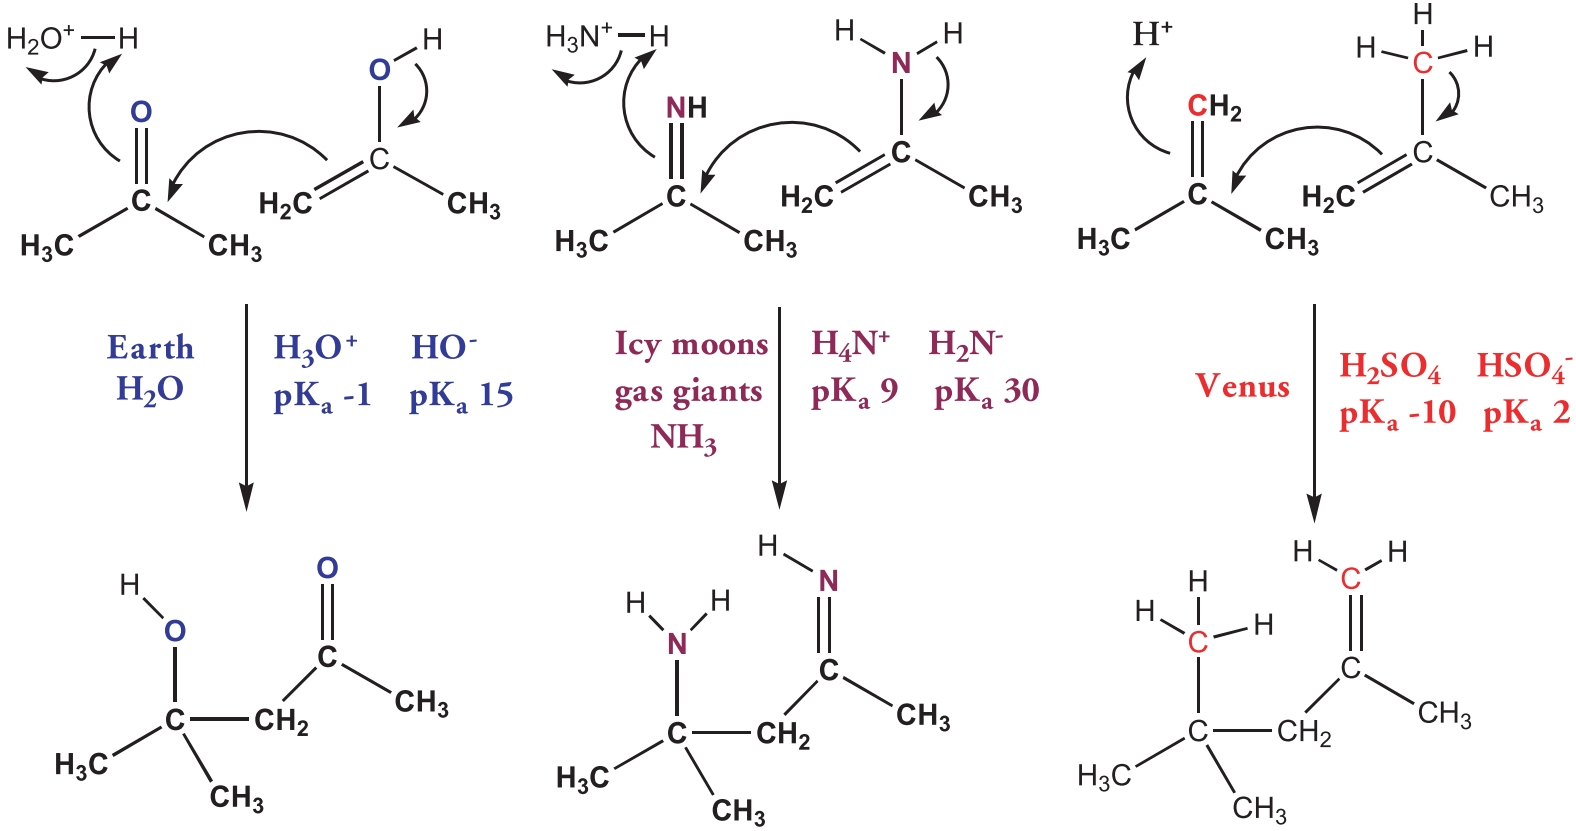
\includegraphics[width=0.9\textwidth]{NoWater}
\end{figure}

\begin{figure}[H]
	\caption{No water? Non-polar solvents}\label{fig:non:polar}
	\begin{subfigure}[t]{0.5\textwidth}
		\caption{Titan--liquid ethane/methane--very cold}
		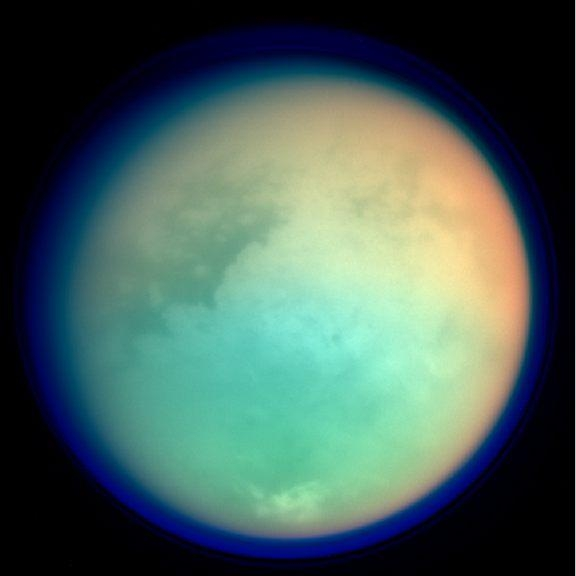
\includegraphics[width=\textwidth]{Titan}
	\end{subfigure}
	\begin{subfigure}[t]{0.5\textwidth}
		\caption{Io--liquid sulfur--Hotter than Earth}
		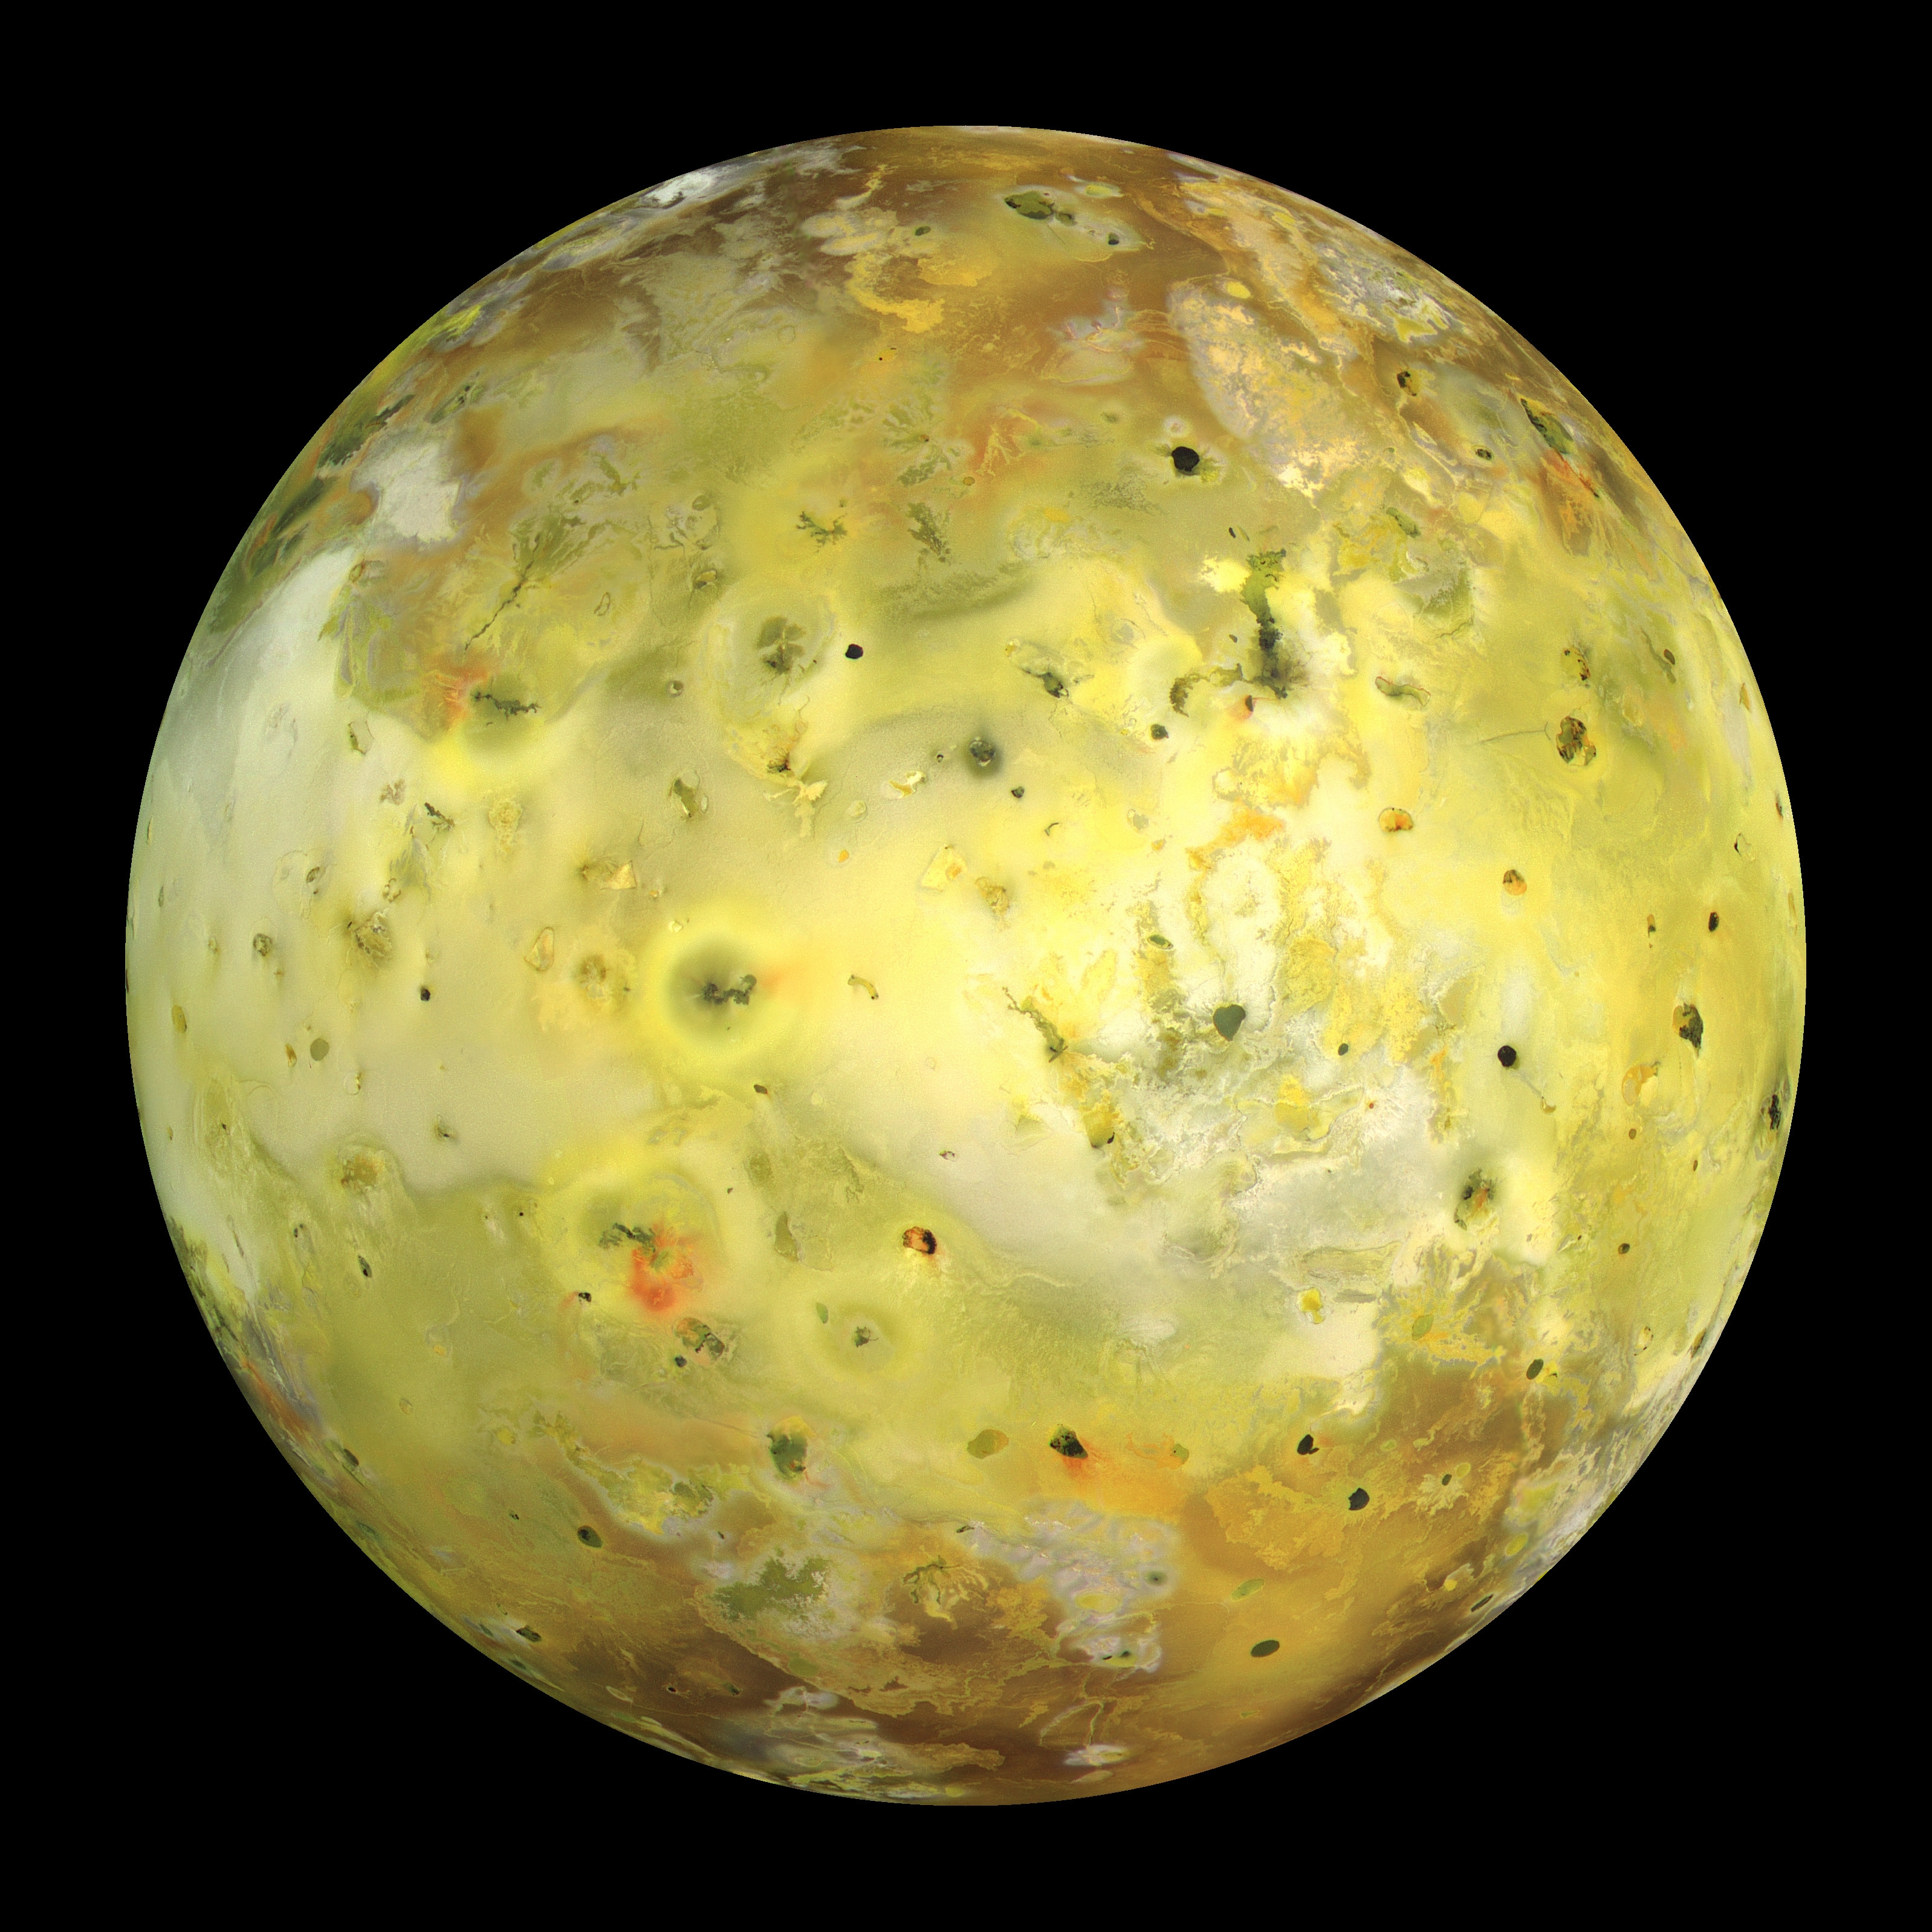
\includegraphics[width=\textwidth]{Io}
	\end{subfigure}
\end{figure}

Open Questions

\begin{itemize}
	\item What other substrates could life exist in?
	\item Would we recognize it?
\end{itemize}

\section[Earth's Early Atmosphere]{Earth's Early Atmosphere--Jim Kasting}

\subsection{Strongly and weakly reducing atmospheres}

\subsubsection{Strongly reducing atmospheres}
\begin{itemize}
	\item Alexander Oparin proposed in his 1924 book, reprinted in English in 1938, that Earth’s early atmosphere was a mixture of highly reduced gases, like methane $(CH_4)$ and ammonia$(NH_3)$\cite{oparin1957origin}
	\item This is similar to how carbon and nitrogen appear in the atmospheres of Jupiter--Figure \ref{fig:Jupiter-galileo}--and Saturn.
	\item In 1953, Stanley Miller, 	working in Harold Urey’s lab at Univ. of Chicago, showed	that plausible prebiotic precursor compounds (e.g.,	amino acids) could be formed by spark discharge\cite{miller1959organic}--Figure \ref{fig:miller_urey3}
	\item Jupiter and Saturn have strong gravitational fields, which keep hydrogen from escaping. Miller argued that the Earth would also have had hydrogen until it had time to escape. 
\end{itemize}

\begin{figure}[H]
	\caption{Strongly reducing atmospheres}
	\begin{subfigure}[b]{0.45\textwidth}
		\centering
		\caption{Jupiter (from Galileo)}\label{fig:Jupiter-galileo}
		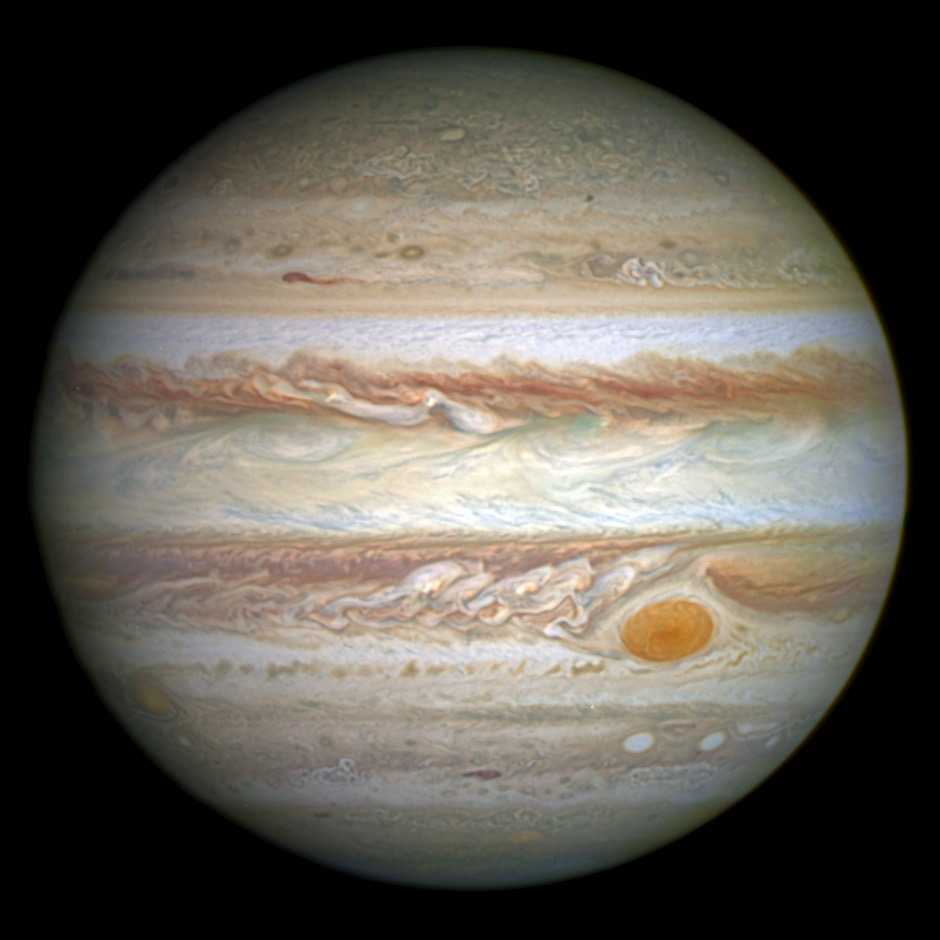
\includegraphics[width=0.8\textwidth]{Jupiter-galileo}
	\end{subfigure}
	\begin{subfigure}[b]{0.45\textwidth}
		\centering
		\caption{Miller-Urey Experiment}\label{fig:miller_urey3}
		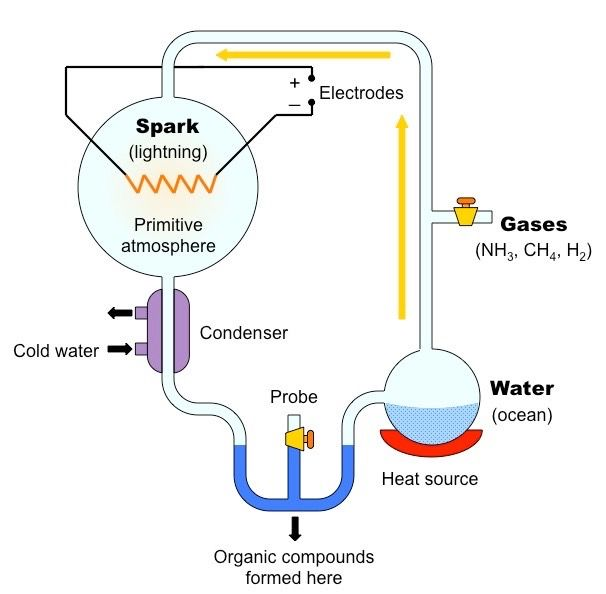
\includegraphics[width=0.8\textwidth]{MillerUrey3}
	\end{subfigure}
\end{figure}

\subsubsection{Weakly reducing atmospheres}
\begin{itemize}
	\item William Rubey, working at the same time as Miller and Urey, noted that the gases being emitted by modern volcanoes--Figure \ref{fig:volcano}-- are not methane and ammonia, but rather $CO_2$, $H_2O$, $N_2$, and $SO_2$, along with minor amounts of $H_2$ and $CO$\cite{rubey1951geologic}.
	\item These gases are relatively oxidized, although free oxygen is absent.
	\item The reason is that Earth’s mantle is partially oxidized: it 	contains some ferric iron ($Fe^{+3}$) in addition to ferrous iron ($Fe^{+2}$). Metallic iron ($Fe^0$) has migrated to the core \cite{wade2005core}
	\item One can simulate the 	resulting atmosphere using a one-dimensional (globally 	averaged) photochemical model--Figure \ref{fig:kasting}

\end{itemize}

\begin{figure}[H]
	\caption{Weakly reducing atmospheres}
	\begin{subfigure}[b]{0.45\textwidth}
		\centering
		\caption{William Rubey, working at the same time as Miller and Urey, noted that the gases being emitted by modern volcanoes are not $CH_4$ and $NH_3$, but rather $CO_2$, $H_2O$, $N2$, and $SO_2$, along with minor amounts of $H_2$ and $CO$}\label{fig:volcano}
		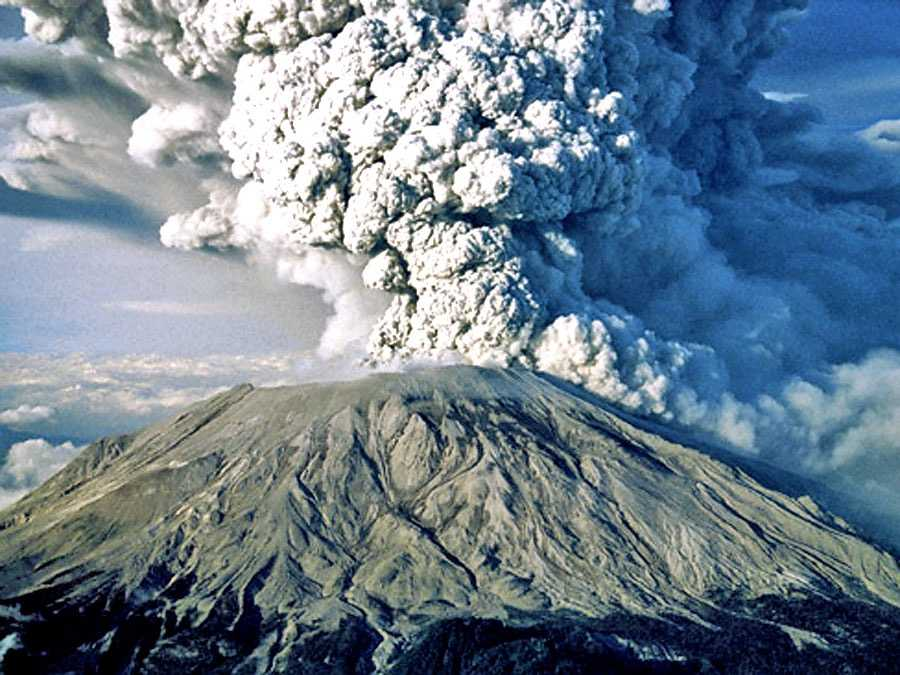
\includegraphics[width=\textwidth]{volcano}
	\end{subfigure}
	\begin{subfigure}[b]{0.45\textwidth}
		\centering
		\caption{Atmospheric Simulation\cite{kasting1993earth}
			A 1-bar atmosphere is assumed, although this need not be the case.
			CO and O are formed by photolysis of $CO_2$. O atoms are then recombined to form $O_2$.
			The $H_2$ concentration is determined, to first order, by 	balancing volcanic outgassing with escape to space}\label{fig:kasting}
		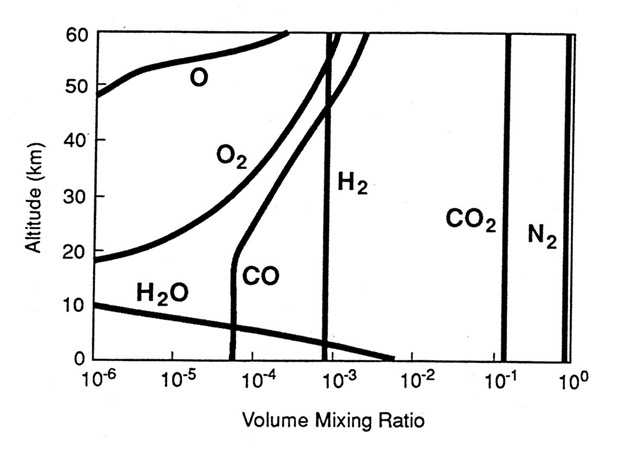
\includegraphics[width=\textwidth]{kasting}
	\end{subfigure}
\end{figure}

\subsection{The faint young Sun problem}

\begin{itemize}
	\item The $CO_2$ content of the atmosphere of Figure \ref{fig:kasting} is 0.2 bar. This is 	just enough to compensate for reduced solar luminosity
	\item The Sun is thought to have been $\approx30\%$ dimmer when it
	formed 4.6 b.y. ago \cite{gough1981solar}
	\item Question: Why was the young Sun less bright?
	\begin{itemize}
		\item Answer: It fuses H into He in its core. The core becomes 	denser, causing it to contract 	and heat up. This makes the fusion reactions proceed faster.
		\item If Earth’s atmospheric composition had not changed with time, the oceans would 	have been frozen over prior to 2 Gya, as first pointed out by Sagan and Mullen \cite{sagan1972earth}
	\end{itemize}
\end{itemize}
\begin{figure}[H]
	\caption[Temperature of Earth]{Temperature of Earth after \cite{kasting1988climate}. Model assumes that proportions of greenhouse gases in early atmosphere match present day atmosphere, so differences are attributable the the Sun. Geologists know that can't be true, as the oceans would have frozen: there is evidence of liquid water from 3.8Gya. We know that Carbon dioxide builds up when temperatures low, so early Earth was probably rich in carbon dioxide. $S$ is solar luminosity, $S_0$ is the present day value of $S$, $T_e$ is effective radiating temperature (energy balance), and $T_S$ is effective surface temperature from climate model.}
	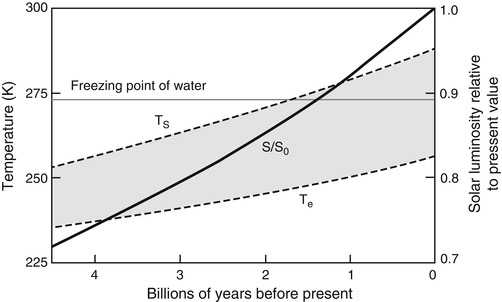
\includegraphics[width=0.8\textwidth]{faint-youg-sun}
\end{figure}

\subsection{The origin of life}

What does all this imply about the origin of life? Origin of life theories fall into three basic categories
\begin{itemize}
	\item Information first (sometimes called ‘RNA first)
	\item Metabolism first
	\item Vesicles first
\end{itemize}
In reality, all three things need to come together. 

We'll focus on metabolism. Environments are also important. Two possibilities are:
\begin{itemize}
	\item  a surface environment--Figure \ref{fig:DarwinsWarmLittlePond}, or 
    \item alkaline (off-axis) midocean ridge hydrothermal vents--Figure \ref{fig:lost_city_vent_field}
\end{itemize}

\begin{figure}[H]
	\caption{Environments are also important}
	\begin{subfigure}[t]{0.45\textwidth}
		\centering
		\caption{Darwin's Warm Little Pond}\label{fig:DarwinsWarmLittlePond}
		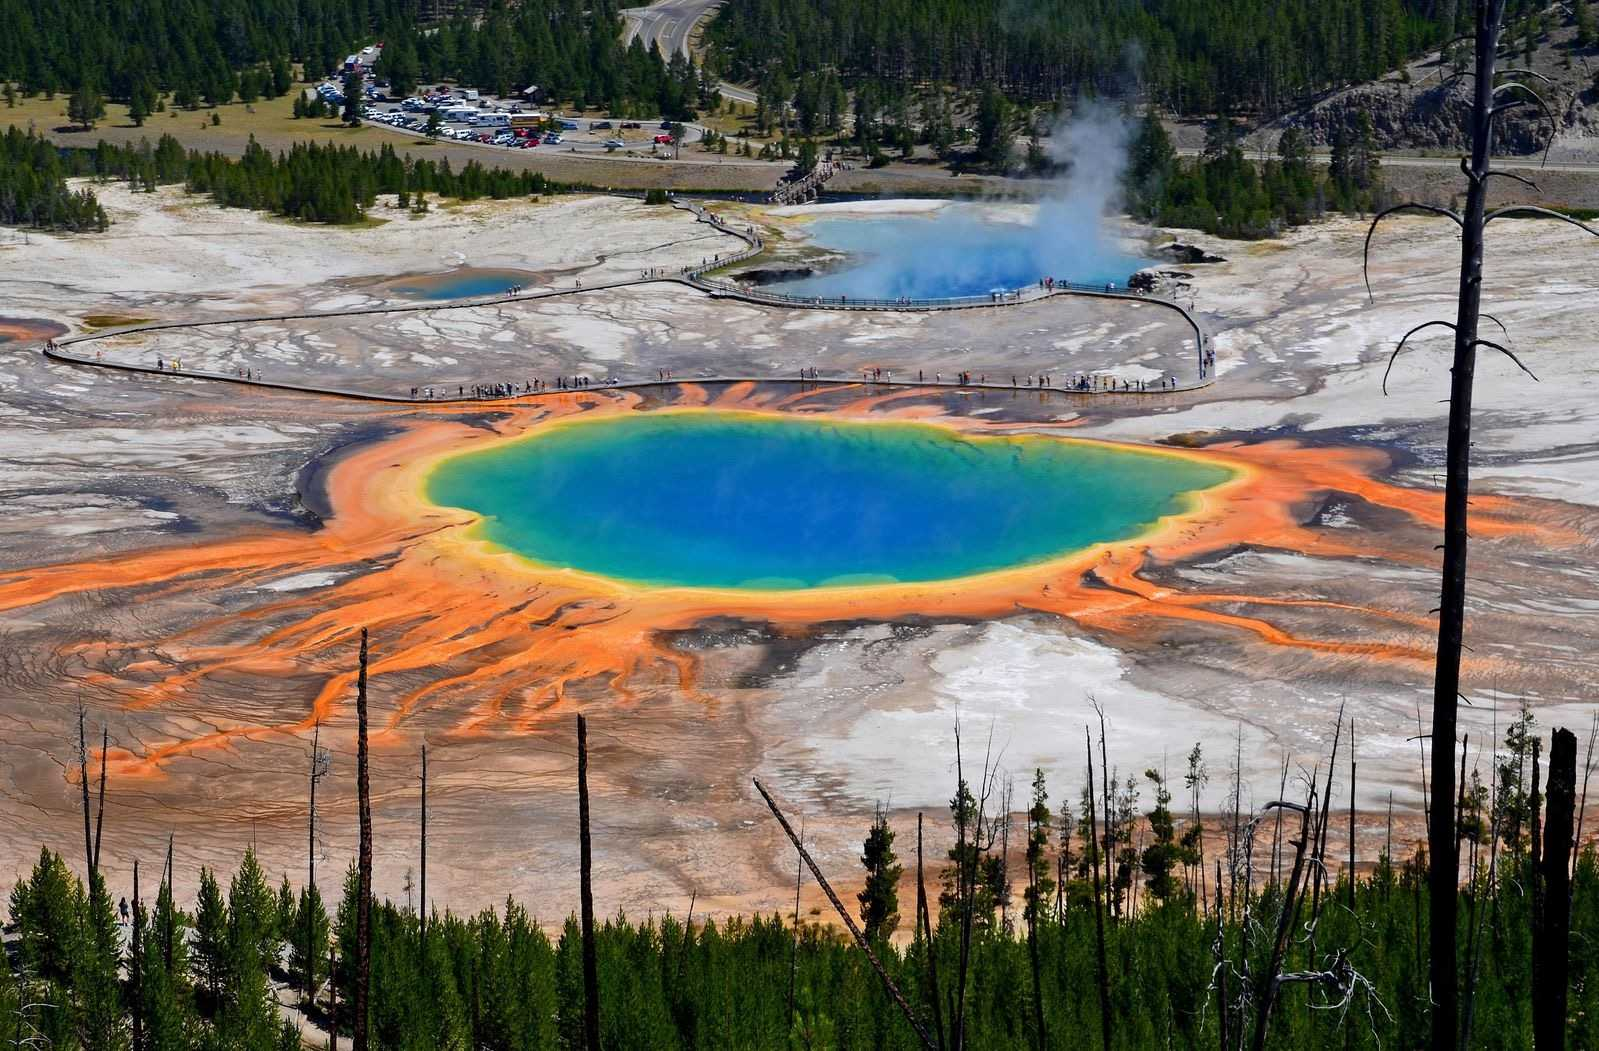
\includegraphics[width=0.8\textwidth]{DarwinsWarmLittlePond}
	\end{subfigure}
	\begin{subfigure}[t]{0.45\textwidth}
		\centering
	\caption{The Lost City vent field on the Midatlantic
	Ridge}\label{fig:lost_city_vent_field}
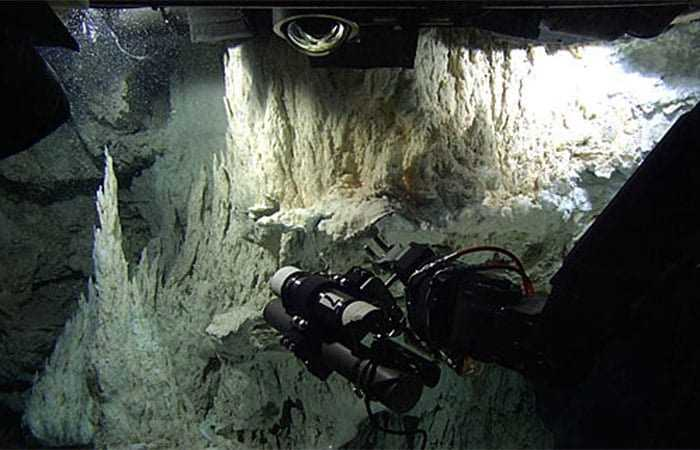
\includegraphics[width=\textwidth]{lost_city_vent_field}
	\end{subfigure}
\end{figure}

\begin{itemize}
	\item Proponents of the ‘Metabolism first’ hypothesis e.g. \cite{russell2006onset} have focused on the alkaline hydrothermal vent environment--Figure \ref{fig:lost_city_vent_field}--not Black Smokers
	\item \Gls{gls:free:energy} can be obtained by 	using $H_2$ to reduce $CO_2$ to	acetate (shown here as acetic 	acid)
	$2 CO_2 + 4 H_2 \rightarrow CH_3 COOH + 2 H_2O$
	\item Additional \Gls{gls:free:energy} is 	available from pH gradients
	\item Quoted \Gls{gls:free:energy} gradients are in the range of -40 to -80 	kJ/mol
\end{itemize}


\begin{itemize}
	\item But \Gls{gls:free:energy} can also be obtained in the surface environment, given a weakly reducing atmosphere--Figure \ref{fig:kasting}
	\item CO is abundant in such an atmosphere due to photolysis of $CO_2$. $H2$ is relatively scarce 	due to escape of hydrogen to space. Thus, the water-gas shift reaction is energetically favourable by ~20 kJ/mol-\cite{kasting2014atmospheric}
	$$CO + H_2O(liquid)\rightarrow CO_2 + H_2$$ 
	\item Consider the reaction $$CO + H_2O(liquid)\rightarrow CO_2 + H_2$$ 
	\item The \Gls{gls:gibbs-free} 	change for this reaction can be written as
	$$\Delta G_R = \Delta G_R^0 + RT \ln{Q}$$ where $$Q=\frac{pH_2.pCO_2}{pCO}$$
	\item Here, $\Delta G_R^0$ is the 	\Gls{gls:free:energy} change at standard state, Q is the
	reaction quotient, and pX represents the partial 	pressure of gas X in bar
	\item For the atmosphere shown here, at $25^{\circ} C$, $RT \ln{Q} \approx 3 KJ/Mol$
	\item Thus, $\Delta G_R \approx -17 kJ/mol$
	\item But the atmosphere shown 	here is a hypothetical early Archean atmosphere, 	appropriate for, say, 3.8 Ga. Hadean atmospheres could 	have been much more CO-rich as a result of impacts \cite{kasting1990bolide} or charged particle bombardment from the young Sun (work in progress)
	\cite Under these Hadean conditions, pCO could have been equal to $pCO_2$, yielding $RT \ln{Q} \approx -20 KJ/mol$ and $\Delta G_R \approx - 40 kJ/mol$.
	\cite This is comparable to \gls{gls:free:energy} gradients suggested for the hydrothermal vent environment \cite{kasting1993earth}
\end{itemize}

Possible advantages of originating life in a surface environment:
\begin{enumerate}
	\item Temperatures may have been cooler, at least in some regions, thereby promoting the stability of nucleic and amino acids
    \item Vesicles composed of simple lipids (as opposed to today’s complex phospholipids) would have been more stable in a freshwater environment
\end{enumerate}

\subsection{Summary}
\begin{itemize}
	\item Earth’s early atmosphere was 	probably a weakly reduced 	mixture of $CO_2$, $H_2O$, and $N_2$ with lesser amounts of $H_2$.
	\item High $CO_2$ levels are needed to resolve the faint young Sun 	problem 
	\item CO levels could have been high during the Hadean as a consequence of impacts and 	charged particle bombardment
	\item The surface environment could have provided substantial \gls{gls:free:energy}	gradients to drive the origin of life, along with relatively cool temperatures and freshwater 	environments in which simple lipid vesicles could have been 	stable
\end{itemize}
% end of text 

% glossary: may need command makeglossaries.exe origins1
\printglossaries

% bibliography goes here
 
\bibliographystyle{unsrt}
\addcontentsline{toc}{section}{Bibliography}
\bibliography{origins,wikipedia}


\end{document}
